% arara: xelatex
% arara: xelatex
% arara: xelatex

% options:
% thesis=B bachelor's thesis
% thesis=M master's thesis
% czech thesis in Czech language
% english thesis in English language
% hidelinks remove colour boxes around hyperlinks

\documentclass[thesis=M,english]{prefs/FITthesis}[2019/03/06]

% \usepackage{subfig} %subfigures
% \usepackage{amsmath} %advanced maths
% \usepackage{amssymb} %additional math symbols

\usepackage[utf8]{inputenc}

\usepackage{graphicx} %graphics files inclusion
% \usepackage{amsmath} %advanced maths
% \usepackage{amssymb} %additional math symbols

\usepackage{dirtree} %directory tree visualisation
\usepackage{subfig} %image side by side
\usepackage{todonotes} %todo
\usepackage{url}
\usepackage{textcomp} %degree symbol
\usepackage{color, colortbl} %color, table color
\usepackage{enumitem} %lists
\usepackage{float} %for H option in figures
\usepackage{array} %table aligment       
\usepackage{amsmath} %cases
\usepackage{amssymb}
\usepackage{svg} %svg
\usepackage{scrextend}
\usepackage{multirow}
\usepackage[ruled,vlined]{algorithm2e}
\addtokomafont{labelinglabel}{\sffamily}


\definecolor{LightCyan}{rgb}{0.88,1,1}
\definecolor{Blue}{rgb}{0.30980, 0.50588, 0.73725}
\definecolor{White}{rgb}{1, 1, 1}

% list of acronyms
\usepackage[acronym,nonumberlist,toc,nopostdot,numberedsection=autolabel,nomain]{glossaries}
\makeglossaries
\newcommand{\tg}{\mathop{\mathrm{tg}}} %cesky tangens
\newcommand{\cotg}{\mathop{\mathrm{cotg}}} %cesky cotangens

% % % % % % % % % % % % % % % % % % % % % % % % % % % % % % % % % % % 
% % % % % % % % % % % % % % % % % % % % % % % % % % % % % % % % % % % 
\department{Department of Applied Mathematics}
\title{Vehicle Routing Problem with Time Windows solved via Machine Learning and Optimization Heuristics}
\authorGN{Adam} %author's given name/names
\authorFN{Zvada} %author's surname
\authorWithDegrees{Bc. Adam Zvada} %author's name with academic degrees
\author{Adam Zvada} %author's name without academic degrees
\supervisor{doc. Ing. Pavel Kordík, Ph.D.}
\acknowledgements{TODO}
\abstractCS{TODO}
\abstractEN{TODO}
\placeForDeclarationOfAuthenticity{Prague} %where you have signed the declaration
\keywordsCS{TODO\newpage}
\keywordsEN{TODO}
\declarationOfAuthenticityOption{5} %select as appropriate, according to the desired license

\newacronym{ai}{AI}{artificial intelligence}
\newacronym{vrp}{VRP}{vehicle routing problem}
\newacronym{cvrp}{CVRP}{capacitated vehicle routing problem}
\newacronym{vrptw}{VRPTW}{vehicle routing problem with time windows}
\newacronym{tsp}{TSP}{traveling salesman problem}
\newacronym{ml}{ML}{machine learning}
\newacronym{pdp}{PDP}{Pick and Deliver}
\newacronym{vrppd}{VRPPD}{vehicle routing problem with pick and deliver}
\newacronym{rl}{RL}{reinforcement learning}
\newacronym{mha}{MHA}{Multi-head Attetntion}
\newacronym{gat}{GAT}{Graph Attention Network}
\newacronym{gcn}{GCN}{Graph Convolution Networks}

\newacronym{ctu}{CTU}{Czech Technical University}
\newacronym{cpu}{CPU}{central processing unit}
\newacronym{cv}{CV}{computer vision}
\newacronym{dex}{DEX}{Deep EXpectation}
\newacronym{dl}{DL}{deep learning}
\newacronym{dlt}{DLT}{Direct Linear Transform}
\newacronym{dsae}{DSAE}{deep sparse autoencoders}
\newacronym{fast r-cnn}{Fast R-CNN}{fast region-based convolutional network}
\newacronym{faster r-cnn}{Faster R-CNN}{faster region-based convolutional network}
\newacronym{fce}{FCE}{Faculty of Civil Engineering}
\newacronym{fit}{FIT}{Faculty of Information Technology}
\newacronym{fn}{FN}{false negatives}
\newacronym{fp}{FP}{false positives}
\newacronym{fps}{FPS}{frames per second}
\newacronym{gige}{GigE}{Gigabit Ethernet}
\newacronym{gpu}{GPU}{graphics processing unit}
\newacronym{hog}{HOG}{histogram of oriented gradients}
\newacronym{hsv}{HSV}{hue-saturation-value}
\newacronym{idsw}{IDSW}{identity switches}
\newacronym{improlab}{ImproLab}{Image Processing Laboratory}
\newacronym{iou}{IoU}{intersection over union}
\newacronym{lbp}{LBP}{local binary pattern}
\newacronym{lstm}{LSTM}{long short-term memory}
\newacronym{mae}{MAE}{mean absolute error}
\newacronym{ml}{ML}{machine learning}
\newacronym{mlp}{MLP}{multi layer perceptron}
\newacronym{mot}{MOT}{multiple object tracking}
\newacronym{mota}{MOTA}{multiple object tracking accuracy}
\newacronym{motp}{MOTP}{multiple object tracking precision}
\newacronym{mots}{MOTS}{multiple object tracking and segmentation}
\newacronym{mp}{MP}{megapixel}
\newacronym{mtmct}{MTMCT}{multi-target multi-camera tracking}
\newacronym{nms}{NMS}{non-maximum suppression}
\newacronym{nn}{NN}{neural network}
\newacronym{pca}{PCA}{principal component analysis}
\newacronym{r-cnn}{R-CNN}{region-based convolutional network}
\newacronym{reid}{ReID}{re-identification}
\newacronym{rgb}{RGB}{red-green-blue}
\newacronym{roi}{RoI}{region of interest}
\newacronym{rmse}{RMSE}{root-mean-square error}
\newacronym{rnn}{RNN}{recurrent neural network}
\newacronym{rpn}{RPN}{region proposal network}
\newacronym{sdk}{SDK}{software development kit}
\newacronym{sift}{SIFT}{Scale-invariant feature transform}
\newacronym{sort}{SORT}{simple online and real-time tracking}
\newacronym{ssd}{SSD}{single-shot detector}
\newacronym{ssr}{SSR-Net}{Soft Stagewise Regression Network}
\newacronym{surf}{SURF}{Speeded-Up Robust Features}
\newacronym{spp}{SPP}{spatial pyramid pooling}
\newacronym{svm}{SVM}{support vector machine}
\newacronym{yolo}{YOLO}{you only look once}


\begin{document}
    \begin{introduction}
    The \gls{vrp} is one of the most extensively studied combinatorial problems. It is easy to define but very difficult to solve\cite{time-complexity-vrp}. The reason \gls{vrp} is attracting many researchers is the fact that finding a near-optimal solution in a reasonable time would have a great impact on many industries, especially in the domain of transportation and logistics. 
    
    \begin{figure}[ht]
        \centering
        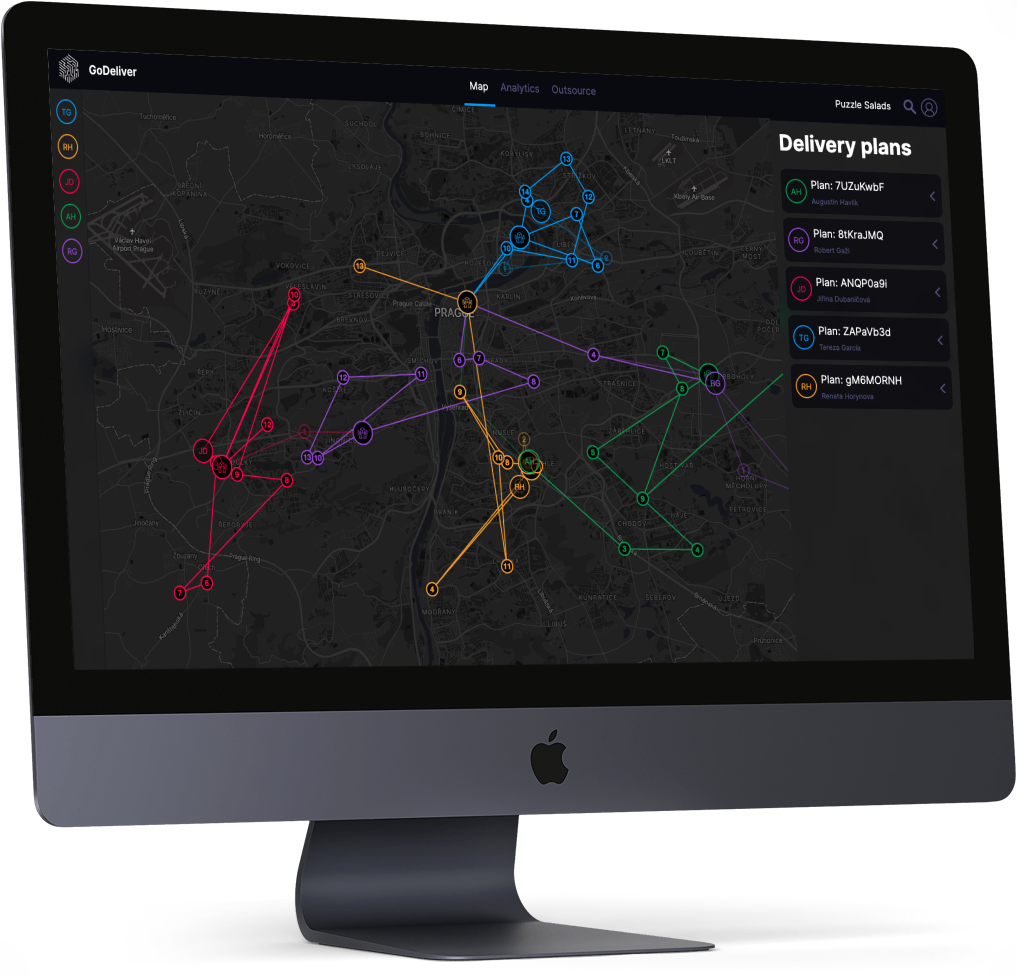
\includegraphics[width=0.5\textwidth]{resources/intro/godeliver-dashboard.png}
        \caption{GoDeliver dashboard visualizing solution for an instance of vehicle routing problem with time windows.}
        \label{fig:godeliver_dashboard}
    \end{figure}
    
    \section{Motivation}
    The paradigm shift in logistics business models towards instant gratification of customers are pushing the planning systems to be flexible and dynamic. The environment is constantly changing and planning systems have to update or entirely replan the instance in a short amount of time but maintaining the best delivery efficiency. Having a powerful planning system results in a dramatic reduction of delivery expanses.
    
    \section{Challenges}
    In the real world, the general VRP problem is not enough to solve the business-related problems. \gls{vrp} has multiple variants adding various constraints such as capacity, demand or time windows for given set of customers. The \gls{vrptw} is main focus of this thesis and we will be looking at some novel approaches how to solve it with \gls{ai}.
    
    \section{Assumptions} 
    We expect that leveraging \gls{ai} or \gls{ml} techniques to solve \gls{vrp} would lead in a drastic reduction of computational time for solving given instance of \gls{vrp}. Moreover, the time complexity would not be exponentially increasing with the problem size. The trade-off lays in the required time to allow \gls{ai} to train and learn how to solve the problem of vehicle routing.
    
    \section{Thesis structure}
    The rest of this thesis is organized as follows:
    \begin{itemize}
        \item Chapter \ref{introduction_vrp} presents a formal introduction to Vehicle Routing Problem.
        \item Chapter \ref{theoretical_background} provides an advanced theoretical background.
        \item Chapter \ref{vrptw-optimization} describes solutions of \gls{vrptw} for optimization heuristics.
        \item Chapter \ref{system} describes how a delivery planning system works.
        \item Chapter \ref{vrptw-ai} describes the proposed method for solving \gls{vrptw} via deep learning.
        \item Chapter \ref{evaluation} evaluates and benchmarks the proposed deep learning model.
    \end{itemize}
\end{introduction}
    \chapter{Introduction to Vehicle Routing Problem}\label{introduction_vrp}

    The problem objective of \gls{vrp} is simply finding the shortest route for multiple vehicles to serve all the given set of customers. The shortest route can be differently interpreted based on your minimalization criteria, e.g, traveled distance, time, or a combination of both. It was first proposed by Dantzig and Ramser \cite{truck-dispatching-problem} in 1959, and since then researchers are coming up with different approaches how to solve the problem. 

    \section{Vehicle Routing Problem Definition}
    
    The general \gls{vrp} can be defined as a problem in a complete graph $G=(V,E)$ of finding the optimal permutation $\pi_l = (\pi_0, \cdots, \pi_m)$ of nodes $V$ all starting from a node $v_0$ for given number of paths $k$ which results in minimal traversal cost where $\forall v \in (V \setminus v_0)$ are visited only once. \gls{vrp} is generalization of \gls{tsp} which only has one path.
    
    \begin{figure}[ht]
        \centering
        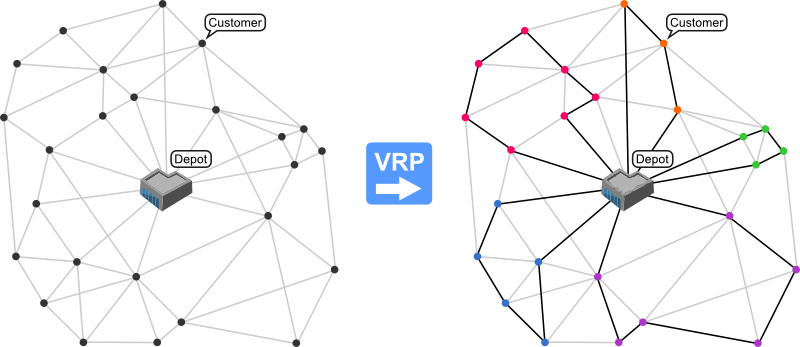
\includegraphics[width=0.75\textwidth]{resources/intro/vrp-graph.png}
        \caption{Intuitive view of \gls{vrp} instance on left and proposed solution for 5 vehicles on the right \cite{vrp-malaga}}
        \label{fig:vrp-graph}
    \end{figure}
    
    \gls{vrp}s are classified as NP-Hard problems which was proved by Lenstra and Kan \cite{time-complexity-vrp}. It means that in the worst case, adding new nodes, i.e., customers results in an exponential increase of computational complexity.
    
    \subsection{VRP Notation}
    Let's introduce our used notation and its real-world interpretation.
    \begin{itemize}
        \item $G=(V,E)$ is a complete undirected graph
        \begin{itemize}
            \item Network of routes
        \end{itemize}
        \item $v_0$ is the initial node
        \begin{itemize}
            \item A depot
        \end{itemize}
        \item $V^{\prime} = (v_1, \cdots, v_n)$ nodes expect the initial node
        \begin{itemize}
            \item Geographically scattered location of customers
        \end{itemize}
        \item $E = \{(v_i, v_j)| v_i, v_j \in V, i \neq j\}$ with associated weight as a cost $c: E \to \mathbb{N}^+$
        \begin{itemize}
            \item A single route between two locations with associated cost, e.g., distance.
        \end{itemize}
        \item $C$ is a matrix of edge weights indexed by nodes. $c_i_j$ where $i,j \in V$
        \begin{itemize}
            \item Matrix of costs between customers
        \end{itemize}
        \item $R_i \subset V$ is a path that starts and ends at $v_0$. $(r_0 = v_0 \land r_{|R_i|} = v_0)$
        \begin{itemize}
            \item Route visit a subset of customers starting and ending at the depot, it can be referred to it as a delivery plan.
        \end{itemize}
        \item $k$ number of paths
        \begin{itemize}
            \item Number of vehicles
        \end{itemize}
        \item $R = R_1, \cdots, R_k$ is a set of paths
        \begin{itemize}
            \item All routes (delivery plans) for a given instance of \gls{vrp}.
        \end{itemize}
        \item $\pi = (\pi_1, \cdots, \pi_k)$ solution for a given instance of \gls{vrp}.
        \begin{itemize}
            \item Customer locations in visiting order for multiple vehicles.
        \end{itemize}
    \end{itemize}
    
    \textbf{Feasibility of \gls{vrp} solution} for \gls{vrp} of routes $R$ is feasible only if each node $V_1$ is visited exactly once.
    
    \textbf{The cost of route $R_i$} which we aim to minimize is the sum of its weights (costs). If we operate in Euclidean space, then it is L2 norm of route locations.
    \begin{equation}
        C(R_i) := \sum_{k = 0}^{|R_i|} c_{r_k}_{r_k+1}
    \end{equation}
    
    \textbf{The cost of \gls{vrp} solution} is the sum of route costs.
    \begin{equation}
        C(R) := \sum_{i = 1}^{|R|} C(R_i)
    \end{equation}
    
\section{Vehicle Routing Flavors}
Our modern world heavily relies on complex logistics networks. It requires to synchronize multimodal planning to ship your goods from one side of the world to your doorstep. In order to achieve this, multiple variants and flavours of \gls{vrp} had to be studied and implemented in the real world use cases. It goes from ordinary variants like measuring the capacity of cars to a more niche problem like eVRP where vehicles are required to make stops to recharge.

All the flavours of \gls{vrp} can be mutually combined, which is usually the main area of research.

    \begin{figure}[ht]
        \centering
        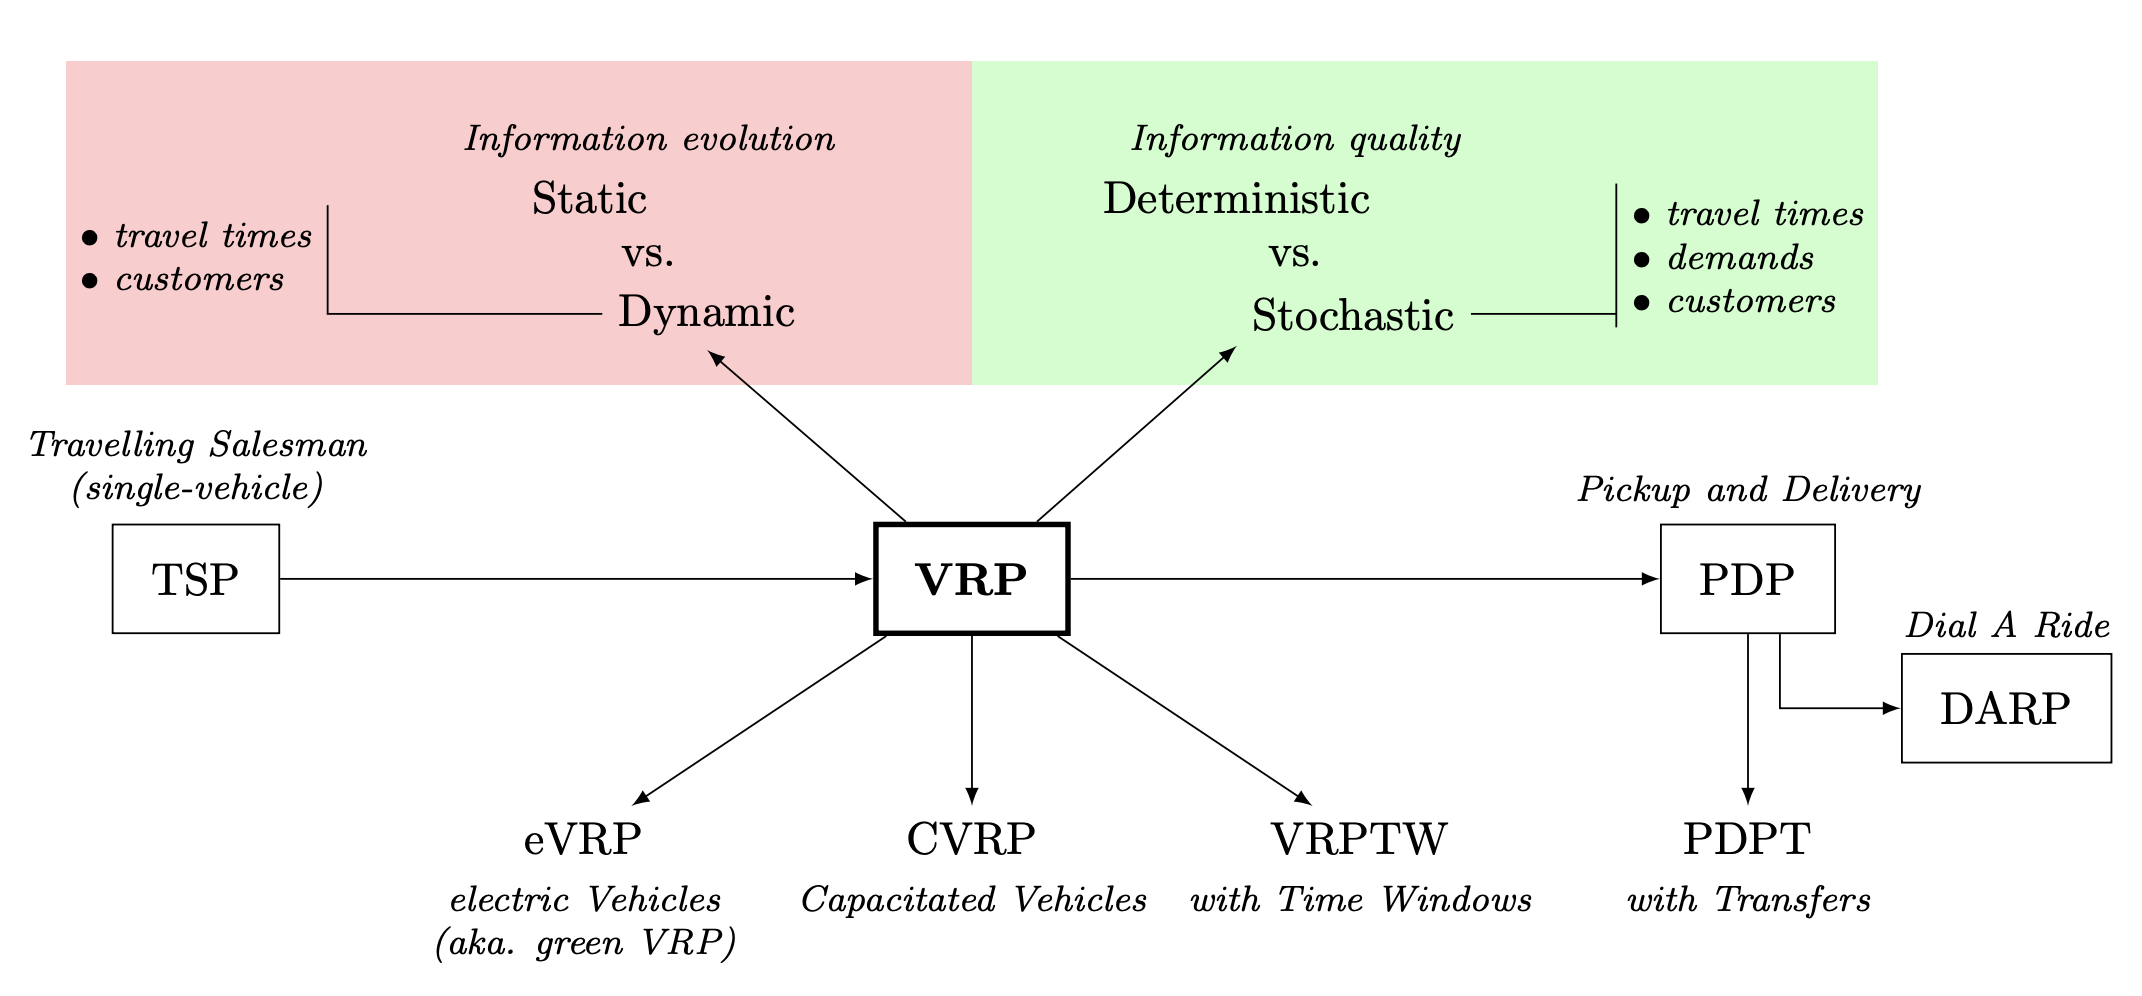
\includegraphics[width=1.0\textwidth]{resources/intro/vrp-flavours.png}
        \caption{Taxonomy of VRPs \cite{bono-stochastic-vrp}}
        \label{fig:vrp-flavours}
    \end{figure}

The sections below are describing each flavour shown in \ref{fig:vrp-flavours}.

    \subsection{Capacitated Vehicle Routing Problem}
    The \gls{cvrp} extends the regular \gls{cvrp} in introducing a capacity element for each customer. In the literature, it is sometimes referred to as a demand. The customer's demand is $d \in \mathbb{N}^+$ which may represent capacity in the form of weight, size but also in some abstract concepts such as a basket of apples. Additionally, each vehicle has a predefined capacity $Q > 0$.
    
    The \gls{cvrp} extends the solution feasibility formula by the following capacity constrain.
    \begin{equation}
        q(R) := \sum_{i \in R} d_i \leq Q
    \end{equation}
    
    If the vehicle capacity of the fleet stays the same, we are dealing with \gls{cvrp} with homogeneous fleet. A fleet with varying capacity for each vehicle is a heterogeneous fleet.
    
    \subsection{Vehicle Routing Problem with Time Windows}
    The \gls{vrptw} \cite{vrptw-solomon} extends the regular \gls{vrp} by time constraint for each customer. Customers have assigned time window interval $[e_i, l_i]$ where $e_li < l_i$. The time interval is the request within a vehicle is supposed to visit the node. 
    
    The time window can be either implemented as a hard constraint or a soft constraint. Hard constraint forces the vehicle to visit the node, i.e., the customer either in the given time interval or the solution is not feasible. Soft constrains are not strictly enforcing the vehicle to visit the customer, but they introduce a penalty for a violated interval barring a penalty cost. The penalty becomes a part of the cost function which \gls{vrp} aims to minimize.
    
    In this thesis, we will be focusing on soft constraints for time windows since it is a better reflection of real world use cases. Most businesses allow couriers to arrive late or early, but these types of arrivals are supposed to be minimized.
    
    \subsection{Pick and Deliver}\label{pick-and-delivery}
    The \gls{pdp} extends the regular \gls{vrp} by pairing pick and drop with precedence relationships, in which a pickup point must precede the paired delivery point. This flavour of \gls{vrp} is one of the most complex and even challenging for conventional methods like optimization heuristics algorithms.
    
    The feasibility of a \gls{pdp} solution is checking whether all delivery points have preceded pickup point.
    
    \subsection{Static vs. Dynamic}\label{dynamic}
    When solving the vehicle routing model, usually we assume that all the input data are static and known with certainty. However, this is not the case in real-life applications where data such as customer demand or travel time are often incomplete or not precise during the planning phase, they are only gradually revealed and specified.
    
    \textbf{Static \gls{vrp}} does not assume that the input data could be subject to change. The \textbf{dynamic \gls{vrp}} is aware about the information evolution\cite{psaraftis} and its goal is to obtain a robust routing planner that will be able to solve already seen instances with subject to small changes without the need of recalculating the whole instance again. This is called a priori optimization, after solving a given instance of a combinatorial optimization problem, it becomes necessary to repeatedly solve many other instances with a small variation from the original instance but without reconsideration of the entire problem \cite{apriori-optimization}.
    
    In this thesis, the \gls{vrp} based on \gls{ai} could be a great candidate for dynamic \gls{vrp} even though, the entire instance is being recalculated. The reason is that the problem solution is calculated in a seconds instead of minutes and the \gls{ai} technically already seen the instance in some variation during the training phase.
    
    Dynamic \gls{vrp} can be achieved with enough robust architecture around the core planner and periodically recalculating the instance with newly revealed information. The planner needs to take its previous solution as an input so the part of the problem does not need to be recalculated. This approach tends to be more exploitative since it is finding a solution in a predefined search space. It would benefit from introducing an explorative element which would diversify the search and could find better cost in a different local optimum.

    \subsection{Deterministic vs. Stochastic}\label{dynamic}
    Psaraftis \cite{psaraftis} stated that there are two important dimensions of input data, the information evolution which is used in dynamic \gls{vrp} and quality of information for stochastic \gls{vrp}. The majority of studied \gls{vrp} models are under the assumption that all the information necessary to formulate the problems is known and readily available. This is true but only for the deterministic settings \cite{vrp-bible}.
    
    A \textbf{\gls{vrp} is stochastic} \cite{stochastic-vrp} when some of its data behave as random variables, and the routes must be defined before the values of these random variables become known. Based on the probability distribution of the random variables, we may extract some hidden information and use it to our advantage in the planning process. The newly created plans will have incorporated stochastic information and the routing decisions may lead to different decisions because of the stochastic information being part of the cost function.
    
    A specific real-life example of stochastic \gls{vrp} would be if we consider an electric fleet of shared mobility vehicles and treat the locations of Blinkee electric scooters as random variables. Based on the probability distribution of Blinkee scooter, we may predict the time and location where a courier will transfer to a new fully charged Blinkee scooter. This action will be incorporated into the planned routes.
    
    In contrast, \textbf{deterministic \gls{vrp}} has no random information which could be leveraged before the execution of routes and all the given information are known with certainty. In this thesis, we are focusing on deterministic \gls{vrp}.
    
    \subsection{Other Flavours}
    Dial-a-Ride (DARP) proposed by Wilson et al. \cite{darp-proposed} in 1971 is a special case of dynamic \gls{vrp} with pick and deliver. Passengers request a ride at a specified origin and drop location with an optional time window. 
    
    \label{split-delivery}Split Delivery \gls{vrp} \cite{split-deliver} is a variant where customers are allowed to be visited more than once. This can be convenient for deliveries of large capacity or stocking fulfillment centers.
    
    Multi Depot \gls{vrp} is a simplification of the vehicle routing problem with pick and deliver, where pick can happen only on predefined depot locations. This simplification of pickup location is making the problems less complex then \gls{vrppd}.
    
\section{VRP in a Real-world}
Consumer habits have been shifting towards online and the pandemic situation only accelerated this process. Delivery option is nowadays taken for granted and consumers are demanding a perfect delivery experience. In 2020, there has been shipped over 5.5 billion packages around the world \cite{num-shipped-packages}.

Solving various flavors of \gls{vrp} efficiently in a reasonable time plays a crucial role for multiple businesses. For example, urban logistics is an essential part of the delivery process, not only it is the last part of the delivery chain, but frequently the courier interacts with the customer and delivery on time with proper ETA prediction is a must. It is also the most expansive part which makes up about 53\% of shipment’s total cost\cite{num-shipped-packages}. Urban logistics by large benefits from a better and more optimized \gls{vrp} which increase the delivery efficiency and reduces the delivery cost.

\begin{figure}[ht]
    \centering
    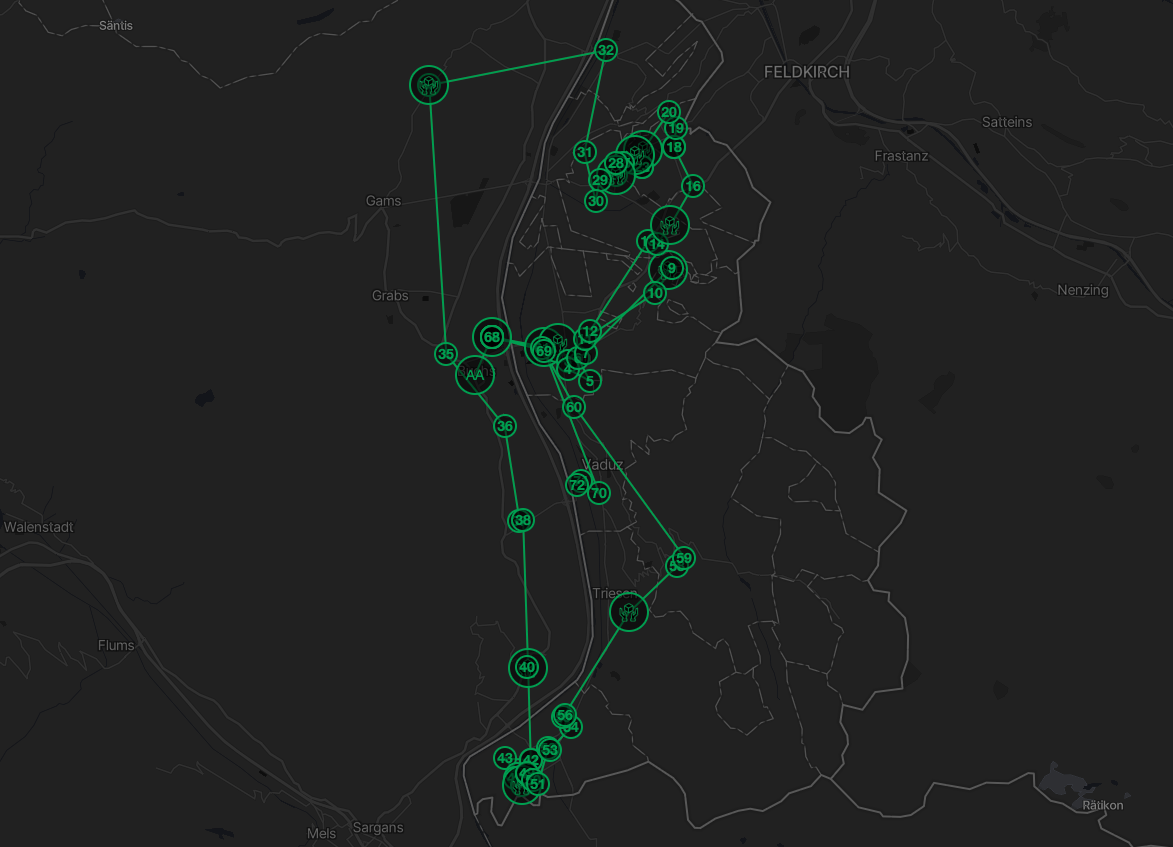
\includegraphics[width=0.75\textwidth]{resources/intro/hofkorb.png}
    \caption{Grocery delivery planning with multiple depots from the GoDeliver system}
    \label{fig:hofkorb}
\end{figure}

At GoDeliver, we are building an autonomous last-mile delivery system and at the core is a planning system which is solving various \gls{vrp}. The flavour which we are focusing on is Dynamic Capacitated Vehicle Routing Problem with Time Windows and Pick and Delivery (CVRPDPTW). GoDeliver typical use case is on-demand food delivery with multiple depots (pick and deliver), this means that the system has to be dynamic and flexible because a new customers are ordering stochastically for a chosen time window. Another our common use case shown in \ref{fig:hofkorb} is grocery delivery with multiple depots, time windows, and capacity for customers.

    \chapter{Theoretical Background}\label{theoretical_background}

In this chapter, we will be covering the advanced theoretical background to fully understand the solved task of \gls{vrptw} using \gls{ai}.

\section{Reinforcement Learning}\label{rl}
    \gls{ml} can be divided with a little simplification into three categories; supervised learning, unsupervised learning, and reinforcement learning. Supervised learning is the most common where the model is learned from the provided labeled data. Unsupervised learning, on the other hand, is about finding a hidden patterns in a collection of data with no labels. Finally, reinforcement learning has no labeled data but learns by interacting with the environment and getting feedback in the form of rewards as shown in Figure \ref{fig:rl-loop}. 
    
    \begin{figure}[ht]
        \centering
        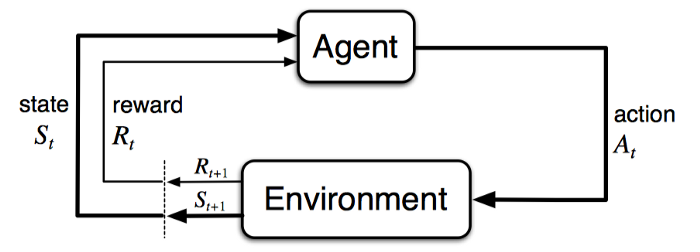
\includegraphics[width=0.75\textwidth]{resources/theoretical-background/rl-loop.png}
        \caption{Agent feedback loop\cite{rl-intro}}
        \label{fig:rl-loop}
    \end{figure}
    
    The Reinforcement Learning mimics the learning process of humans beings. By experiencing the world and accumulating knowledge, we are learning how to handle novel situations. \gls{rl} system consists of agent in observed state $s_t$, the agent interacts with the environment via its actions $a_t$ at discrete time steps $t$ and receives a reward $r_{t+1}$ for given action. The action moves the agent into a new state $s_{t+1}$. The goal of the agent is to learn a policy $\pi$ which chooses the action that maximizes the agent's rewards based on the environment \cite{rl-intro}. 
    
    %The policy is formally defined as a probability distribution of 
    \subsection{State and Action Value Functions}
        Transition to a new state gives us a reward and to maximize it, we need a way to quantify how good a state is. A state-value function $V_{\pi}(s)$ predicts a future reward for a given state when following the policy $\pi$ \cite{rl-intro}. 
    
        \begin{equation}
            V_{\pi}(s) = \mathop{\mathbb{E}}[G_t|S_t = s]
        \end{equation}
        \begin{equation}\label{discount-reward}
            G_t = \sum_{k=0}^{\infty} \gamma^k R_{t+k+1}
        \end{equation}
        The equation \ref{discount-reward} calculates $G_t$, all future rewards, sometimes called as $return$ \cite{rl-intro}. The $\gamma \in [0,1]$is a discount factor and penalizes the rewards in the future, incorporating the possible uncertainty and variance of the future rewards.
    
        We will also define action-value $Q_{\pi}(s, a)$ which is for a similar purpose as state-value function but predicts the reward for action and state following the policy $\pi$.
        \begin{equation}
            Q_{\pi}(s, a) = \mathop{\mathbb{E}}[G_t|S_t = s, A_t = a]
        \end{equation}
        
        The decomposition of state-value and action-value function replays on Bellman equations \cite{bellman-eq}. The decomposition of state-value function is
        \begin{equation}
            V_{\pi}(s) = \mathop{\mathbb{E}}[G_t|S_t = s]
        \end{equation}
        \begin{equation}
            V_{\pi}(s) = \mathop{\mathbb{E}}[R_{t+1} + \gamma R_{t+2} + \gamma^2 R_{t+3} + \cdots |S_t = s]
        \end{equation}
        \begin{equation}
            V_{\pi}(s) = \mathop{\mathbb{E}}[R_{t+1} + \gamma(R_{t+2} + \gamma R_{t+3} + \cdots) |S_t = s]
        \end{equation}
        \begin{equation}
            V_{\pi}(s) = \mathop{\mathbb{E}}[R_{t+1} + \gamma G_{t+1} |S_t = s]
        \end{equation}
        \begin{equation}
            V_{\pi}(s) = \mathop{\mathbb{E}}[R_{t+1} + \gamma V(S_{t+1}) |S_t = s]
        \end{equation}
        Similarly, this method is applicable to action-value function,
        \begin{equation}
            Q_{\pi}(s, a) = \mathop{\mathbb{E}}[R_{t+1} + \gamma V(S_{t+1}) |S_t = s, A_t = a]
        \end{equation}
        \begin{equation}
            Q_{\pi}(s, a) = \mathop{\mathbb{E}}[R_{t+1} + \gamma \mathop{\mathbb{E}}_{a \sim \pi} Q(S_{t+1}, a) |S_t = s, A_t = a]
        \end{equation}
    
        \subsection{Policy Gradients}
        Policy Gradient \cite{policy-gradient} is a method for solving the reinforcement learning problem and learning the policy that maximizes the rewards. We define a set of parameters $\theta$ that directly models the policy, $\pi_{\theta}(a|s)$.
    
        To optimize $\theta$ for the best reward, we define an objective function \cite{policy-gradient} as
        \begin{equation}
            J(\theta) = \sum_{s \in S} d_{\pi_{\theta}}(s)V_{\pi_{\theta}}(s)
        \end{equation}
        where $d_{\pi_{\theta}}(s)$ is stationary distribution of Markov chain for $\pi_{\theta}$, the probability of ending in a given state \cite{markov-bullshit}.
        \begin{equation}
            d_{\pi_{\theta}} = \lim_{t -> \infty} P(S_t = s | s_0, \pi_{\theta})
        \end{equation}
        
        The objective function $J(\theta)$ optimizes the $\theta$ parameters via gradient ascent [TODO]. 
        \begin{equation}
            \theta_{t+1} = \theta_{t} + \alpha \nabla J(\theta_{t})
        \end{equation}
        However, computing $\nabla J(\theta)$ is tricky because it depends on the action selection and the stationary distribution of states \cite{policy-weng}. Policy gradient can be simplified using Policy Gradient Theorem by Sutton et al. \cite{policy-gradient}.
        
        The proof of policy gradient theorem is quite long and complicated, but you may go through it in this article \cite{policy-weng} which is inspired by Sutton and Barto \cite{rl-intro}. Policy gradient is simplified to the form as
        \begin{equation}
            \nabla J(\theta) = \mathop{\mathbb{E}}[ \nabla \ln \pi (a|s, \theta) Q_{\theta}(s, a)]
        \end{equation}
    
        \subsection{REINFORCE}\label{reinforce}
        REINFORCE algorithm proposed by Williams \cite{reinforce} in 1992 is a policy gradient method to update the policy parameter $\theta$.
        
        \begin{algorithm}
        \end{algorithm}
    

    \section{Attention Mechanism}\label{attention}
    TODO    

    \subsection{Transformer}\label{transformer}
    TODO
    
    \subsection{Graph Attention Network}\label{graph-attention-network}
    TODO
    
    


    \chapter{VRPTW via Optimization}


\section{Insertion Heuristics}
TODO
        
\section{Google OR-Tools}
TODO
    
\section{Large Neighborhood Search}
Heuristics based on large neighborhood search have shown superior results in solving a wide variety of routing problems. Large neighborhood search was first introduced by Shaw \cite{shaw-lns} in 1997.

Large neighborhood search is an iterative algorithm that gradually improves its solution by exploring its neighborhoods. The neighborhoods are defined by applying \emph{destroy} and \emph{repair} operator. The destroy operator removes a random part of the solution such that different parts are destroyed in each iteration. The repair operator takes the partial solution and rebuilds into a fully feasible solution \cite{lns}.\newline

In the implementing of large neighborhood search, the most important is to pick the proper degree of destruction for the destroy operator. If it destroys a small part of the solution, then it leads to ineffective exploration of the search space. In the opposite, when destroying large parts of the solution, the algorithm will keep re-optimizaing, which yields poor quality solutions with higher complexity \cite{lns}. The degree of destruction can be either chosen randomly or it can be gradually increased during the execution.\newline

\begin{algorithm}[H]
    \SetAlgoLined
    Initialize a feasible solution $x_b$;
    
        \While{stopping criteria is met}{
    
            $x_t$ = repair(destroy($x_b$));
            
            \If{accept($x_t$, $x$))}{
                Accept a new solution $x = x_t$;
            }
            
            \If{cost($x_t$) $>$ cost($x_b$)}{
                
                Keep the best $x_b = x_t$;
            
            }
        }
        return $x_b$;
    \caption{Large Neighborhood Search}
\end{algorithm}


The original large neighborhood search algorithm only accepted a superior solution based on the cost function. To achieve better exploration, a new acceptance criterium was used, inspired by the algorithm of simulated annealing \cite{lns-anneling}. The algorithm accepts the solution $x$ based on probability $e^{(c(x_t) - c(x))/T}$ where $T$ is the parameter for temperature. The temperature is gradually decreasing resulting in accepting fewer deteriorating solutions.

\subsection{Adaptive Large Neighborhood Search}
Adaptive Large Neighborhood Search is an extension of \gls{lns} that was proposed by Ropke et. al \cite{alns} in 2006.

\gls{alns} supports multiple destroy operators and repair methods.

and insertion operators are selected based on their past performance during the search, usually by employing a roulette wheel selection process with an adaptive weight adjusting mechanism \cite{Azi2014, Gschwind2016, Masmoudi2020}. Ropke and Pisinger (2006) \cite{Ropke2006} used the adaptive large neighborhood search heuristic to solve the PDP with time windows. Their algorithm used removal and insertion operators already existing in the literature, including the removal operator by Shaw (1997) \cite{Shaw1997}, and an acceptance criterion for new solutions known from simulated annealing. The algorithm by Ropke and Pisinger has proven to be powerful and has served as a building block for many further studies in complicated routing problems, particularly PDP and DARP \cite{Gschwind2016, Braekers2016, Masmoudi2016, Belhaiza2017, Drexl2018, Belhaiza2019, Masmoudi2020, Wang2020, Cauchi2020, Malheiros2021}. Gschwind and Drexl (2016) \cite{Gschwind2016} adopted the algorithm from Ropke and Pisinger and added three more removal operators. They also demonstrated how to test a new solution for feasibility in an amortized constant time. Their version of the adaptive large neighborhood search produced better solutions on standard DARP instances compared to the vast majority of other algorithms, except for the hybrid genetic algorithm by Masmoudi et al. (2017) \cite{Masmoudi2017}.
\vspace{0.5cm}

The other well-known category of metaheuristics are population-based methods, which are inspired by natural processes, such as the evolution of species or the behavior of insects. All successful population-based heuristics rely on local search methods to drive the search towards promising areas and to avoid local optima. As a result, the majority of population-based algorithms are naturally hybrid \cite{toth2015vrp}.


\section{Ant Colony Optimization}
This metaheuristic has also proven practical for many routing problems. It is inspired by the pheromone mechanism used by ants for coordination. Each ant simulates a solution by traversing the graph along its edges and accumulates pheromons along the edges it traversed. In each iteration, the ants select the edges with a probability proportional to the pheromon value. The pheromon evaporates after a given number of iterations, so the most promising edges remain at the end \cite{Bono2020, Solnon2010}. The algorithm by Reimann et al. (2004) \cite{Reimann2004} was one of the most successful.
Ant colony optimization algorithm is particularly interesting in dynamic and stochastic settings. When new information is received, such as a new request arrives, or some delays occur, the algorithm uses the pheromone trails from previous iterations. This relies on the assumption that the new information does not disrupt the current solution too much and that some patterns can still be exploited \cite{Schyns2015, Bono2020}.
    \chapter{VRPTW via AI}
In this chapter, we will review the current end-to-end \gls{ai} methods for solving \gls{vrp} and propose our extension for solving \gls{vrptw}.

Machine learning and artificial intelligence have been replacing many hand-engineered algorithms and providing state-of-the-art results. In recent years, reinforcement learning \ref{rl} and advances in attention models \ref{attention} has shown great promise to disrupt the field of heuristics algorithms \cite{rl-constraint-opt, attention-route, dpdp}. Heuristics algorithms \cite{heuristics-algo} are incomplete methods that can compute solutions efficiently, but are not able to prove the optimality of a solution. Most of the business challenges do not require the most optimal exact solution \cite{excat-algo} but focus on approximation of the optimal solution in a reasonable time.

\section{Related Work}
Researchers have been mainly active in solving general \gls{vrp}...
TODO

\section{Solution}
The end-to-end \gls{ai} method pro solving \gls{vrptw} is extension of the work done by Kool et al. \cite{attention-route}. 

Let us describe the high-level concept behind the method. Consider we have a model as blackbox which takes \gls{vrptw} instance as an input and outputs probabilities for all the \gls{vrptw} nodes. The probability represents which node should be visited next and by following to the most probable node we get a partial solution which will be considered by the blackbox. We iterate this process until all nodes have been visited and we acquire a feasible plan as shown on Figure \ref{fig:attention-route-diagram}.

    \begin{figure}[ht]
        \centering
        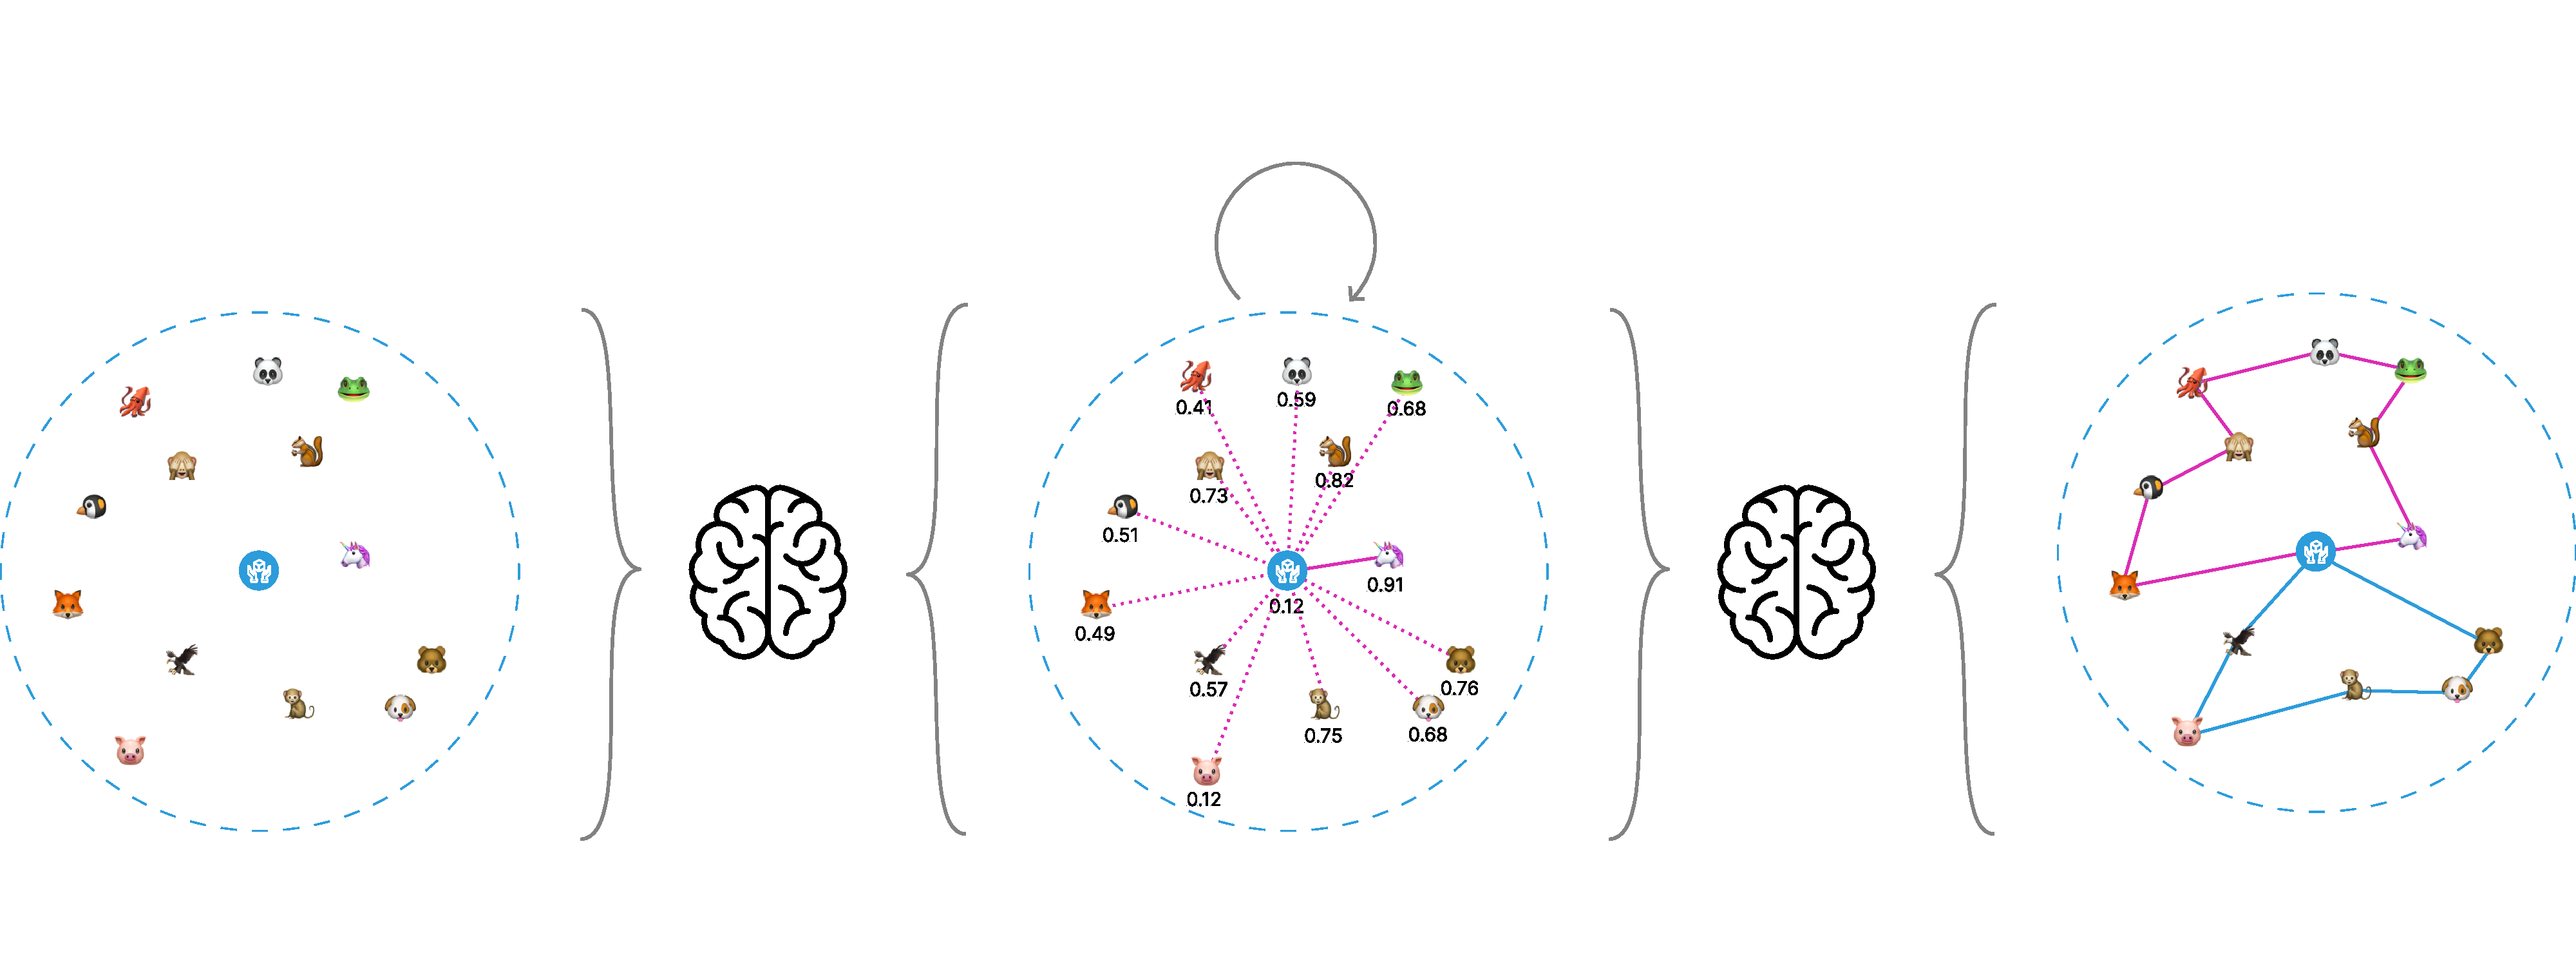
\includegraphics[width=1.0\textwidth]{resources/vrptw-ai/attention-route-diagram.pdf}
        \caption{High-level concept behind the used method.}
        \label{fig:attention-route-diagram}
    \end{figure}

    \subsection{Model Architecture}
    The model architecture \cite{attention-route} leveraging recent advancements in attention mechanism is here extended by the time window constraint. The model is built upon transformers \ref{transformer}, graph attention network \ref{graph-attention-network}, and reinforcement learning \ref{rl}. The network structure is encoder-decoder that fits well for solving sequential decision problems. The structural input instance is extracted by the encoder \ref{vrptw-encoder} and then the solution is incrementally constructed by the decoder \ref{vrptw-decoder}.
    
    The \gls{vrptw} input instance is consisted from:
    \begin{itemize}\label{input-data}
        \item $X = \{x_1, \cdots, x_n\}$ where $x_i$ is two-dimensional coordinates in the euclidean space.
        \item $x_0$ is the location of depot.
        \item $D = \{d_1, \cdots, d_n\})$ is the demand capacity for each of the locations.
        \item $T = \{(e_1, l_1), \cdots, (e_n, l_n)\})$ is time windows for each of the location where $e_i$ is the beginning and $l_i$ is the end of the considered time window.
    \end{itemize}
    
    The output is the solution of VRPTW instance and is represented as a permutation $\pi$ of locations $X \cup x_0$.
    \begin{itemize}
        \item $\pi = \{\pi_1, \cdots, \pi_T\} \in \{x_0, \cdots, x_n\})$ 
    \end{itemize}
    
    \subsubsection{Encoder}\label{vrptw-encoder}
    The encoder uses graph attention network \ref{graph-attention-network} to embed the node features to graph embedding. Then the decoder architecture is the same as the decoder of transformer \ref{transformer}. Typicaly, the decoder of transformer uses positional encoding \cite{positional-encoding} to embed the input, but in this case it has been replace with \gls{gat} \ref{graph-attention-network} since we deal with graph-based structure and the input order does not matter.
    
    The first step is to perform the initial embedding of input data \ref{input-data} via learned linear projections as in \gls{gat}. The $h_{i}^{l}$ represents the node embedding of layer $l \in \{0, \cdots, N\}$ (N=3).
    \begin{equation}
        \widetilde{x} = \text{concat}(X, D, T)
    \end{equation}
    \begin{equation}
        h_{i}^{0} = \begin{cases} W \widetilde{x}_i + b_i &\mbox{if } i > 0 \\ W \widetilde{x}_0 + b_0 & \mbox{if } n = 0 \end{cases}
    \end{equation}
    
    The node embeddings are updated via $N$ attention layers, each containing multi-head attention \ref{multi-head-attention} (M=8) and a fully connected feed-forward network with normalization. The structure is identical to transformer's encoder \ref{transformer} with additional support of graph structure \ref{graph-attention-network} as shown on Figure \ref{fig:encoder-diagram}.
    
    \begin{figure}[ht]
        \centering
        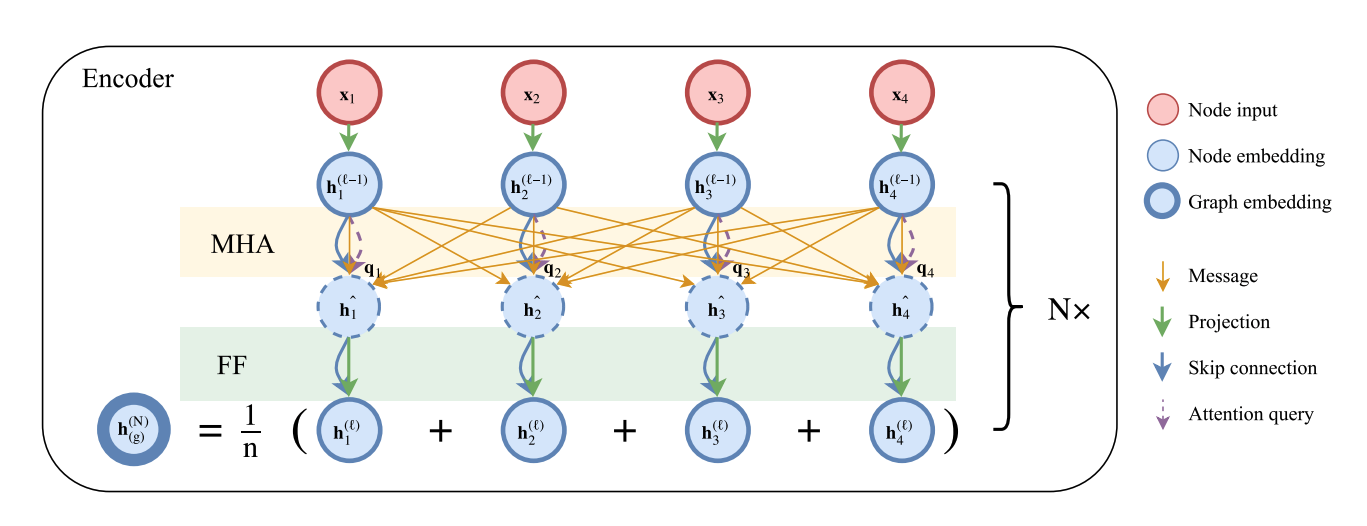
\includegraphics[width=1.0\textwidth]{resources/vrptw-ai/encoder-diagram.png}
        \caption{Encoder layers \cite{attention-route}}
        \label{fig:encoder-diagram}
    \end{figure}
    
    The equation \ref{encoder-qkv} calculates the query $Q$, key $K$ and value $V$ of multi-head attention layer using the node embeddings and weights $W_m^Q$, $W_m^Q$, and $W_m^Q$, respectively. The number of heads is represented by $m \in \{1, \cdots, M\}$ (M=8).
    
    \begin{equation}\label{encoder-qkv}
        \textbf{q}_{im}^l = W_m^Q h_i^(l-1), \textbf{k}_{im}^l = W_m^K h_i^(l-1), \textbf{v}_{im}^l = W_m^V h_i^(l-1)
    \end{equation}
    
    The query and key values are used in calculating the compatibility $u_{ijm}^l$ of node $i$ with a node $j$ \ref{mha-compatibility}. If node $i$ is not adjecnt to node $j$ then they are not compatible and the value is set to a large negative number.
    
    \begin{equation}\label{mha-compatibility}
        u_{ijm}^l = \begin{cases} q_{im}^l k_{jm}^l &\mbox{if $i$ adjacent to $j$} \\ -\infty &\mbox{otherwise} \end{cases}
    \end{equation}
    
    The attention score $a_{ijm}^l \in [0,1]$ is calculated using softmax from the compatibility values of nodes \ref{encoder-attention-score}
    
    \begin{equation}\label{encoder-attention-score}
        a_{ijm}^l = \dfrac{e^{u_{ijm}^l}}{\sum_{j'=0}^n e^{u_{ij'm}^l}}
    \end{equation}
    
    The transformed $h'_{im}^l$ \ref{h-prime} aggregates all attention scores across neighbour nodes, which is based on GAT \ref{graph-attention-network}. 

    \begin{equation}\label{h-prime}
        h'_{im}^l = \sum_{j=0}^n a_{ijm}^l v_{jm}^l
    \end{equation}
    
    Finally, we may calculate the multi-head attention \ref{transformer} for layer $l$ as a function of $\{h_1^{l-1}, \cdots, h_n^{l-1}\}$ through $h'_{im}^l$.
    
    \begin{equation}
        \text{MHA}_i^l(h_1^{l-1}, \cdots, h_n^{l-1}) = \sum_{m=1}^M W_{m}^O h'_{im}^l
    \end{equation}
    
    \begin{equation}
        \widetilde{h}_i = \text{BN}^l(h_i^{l-1} + \text{MHA}_i^l(h_1^{l-1}, \cdots, h_n^{l-1})))
    \end{equation}    
    \begin{equation}
        h_i^l = \text{BN}^l(\widetilde{h}_i + \text{FF}^l(\widetilde{h}_i))
    \end{equation}
    
    In the final layer, the encoder computes the aggregated embedding of the input graph as the mean of the final node embeddings.
    \begin{equation}
        h^N = \dfrac{1}{n} \sum_{i=1}^m h_i^N
    \end{equation}
    
    The output of the encoder's final layer is passed to the decoder, which is detailed in the next sections \ref{vrptw-decoder}.
    
    \subsubsection{Decoder}\label{vrptw-decoder}
    Decoder works sequentially through timestamps $t \in \{0, \cdots, n\}$, at each timestamp one node is selected to be visited based on partial route $\pi_{1:t-1}$. It is predicting the probability distribution over nodes according to the node embedding and context vector of the encoder \ref{vrptw-encoder}.
    
    The decoder uses a new context vector $h_{c}^{'}$ which represents the state \ref{rl} and it goes as follows:
    \begin{equation}\label{decode-state-vec}
        h_{c}^{'} = \begin{cases} \text{concat}(h_N; h_0^N; D_t) & \mbox{if } t = 0 \\ \text{concat}(h_N; h_{\pi_{1:t-1}}^N; D_t) & \mbox{if } t > 0 \end{cases}
    \end{equation}
    The state of $h_{c}^{'}$ is concatenation of $h_N$, the output of the encoder, $h_{\pi_{1:t-1}}^N$, the embedding of previous partial solution, and $D_t$, the remaining demand capacity of the vehicle.
    
    Since the decoder architecture is transformer \ref{transformer} a multi-head attention layers continue and the are resposible for chosing the next node to visite which is defined as an action \ref{rl}.
    
    TODO MHA context embedings + mask with compatibility
    TODO The calculation of compability+ mask with compatibility
    
    The final layer calculates the desired probability $p_{\theta}('pi_t|X, \pi_{1:t-1})$, a logit layer. It is predicted with a single-head attention layer as follows:
    
    \begin{equation}
        q = W^Q h_c, k_j = W^K h_j^N
    \end{equation}
    
    \begin{equation}
        u_j = \begin{cases} C . \text{tanh}(q^T k_{c}) &\mbox{if }  d_j <= D_t \text{ and } x_j \notin \pi_{1:t-1} \\ -\infty &\mbox{otherwise} \end{cases}
    \end{equation}
    
    If we would consider time window as a hard contraint, the calculation of compatibility would have to extended with condition to check fesibility of time windows.
  
    \begin{equation}\label{encoder-attention-score}
        p_{\theta}('pi_t|X, \pi_{1:t-1}) = \dfrac{e^{u_j}}{\sum_{j'=0}^n e^{u_j'}}
    \end{equation}
    
    \begin{figure}[ht]
        \centering
        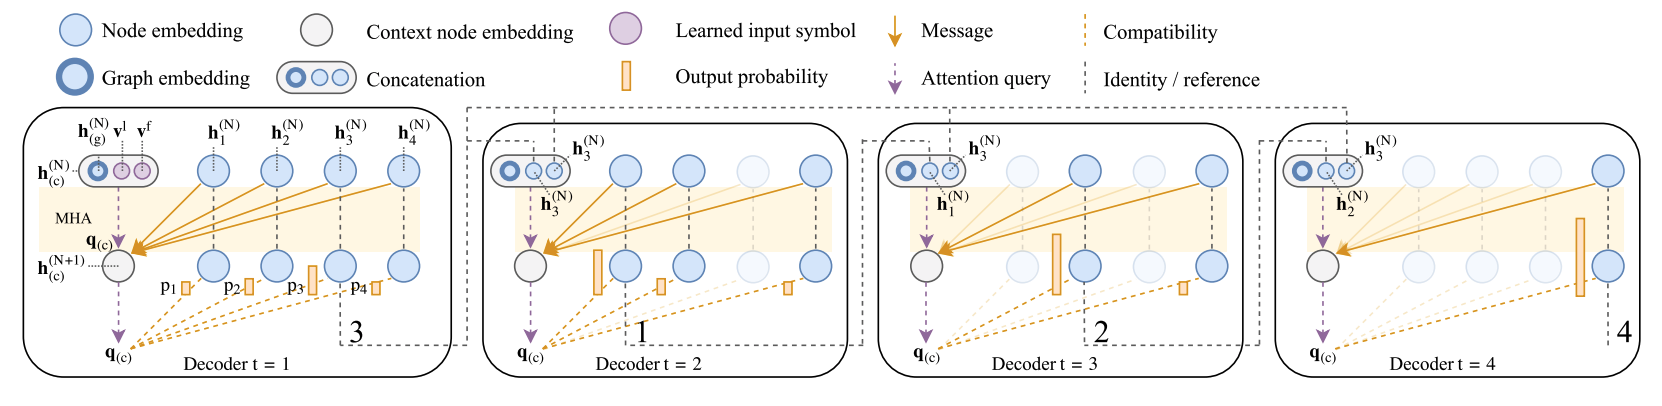
\includegraphics[width=1.0\textwidth]{resources/vrptw-ai/decoder-diagram.png}
        \caption{TODO \cite{attention-route}}
        \label{fig:encoder-diagram}
    \end{figure}
    
    \subsection{Reinforcement Learning}\label{vrptw-rl}
        
    \subsection{Integrating Distance Matrix}
    Multidimensional scaling

    \chapter{Planning System}

In this chapter, take a look at how the GoDeliver\footnote{\url{https://godeliver.co/}} system works and the integration of the \gls{vrptw} \gls{ai} planner.

\section{GoDeliver System}

The GoDeliver system is consisted of multiple services, each responsible for a given subproblem of the delivery process. The core of the system is GoDeliver service, which implements all system APIs and performs the basic CRUD\footnote{Create, read, update and delete} operation on our NoSQL database. The database stores information about business, delivery orders, couriers, and delivery plans. In the Figure \ref{fig:godeliver-system} is visualized the simplified architecture of GoDeliver system, it is especially oriented to show how the planning process works.

\begin{figure}[ht]
    \centering
    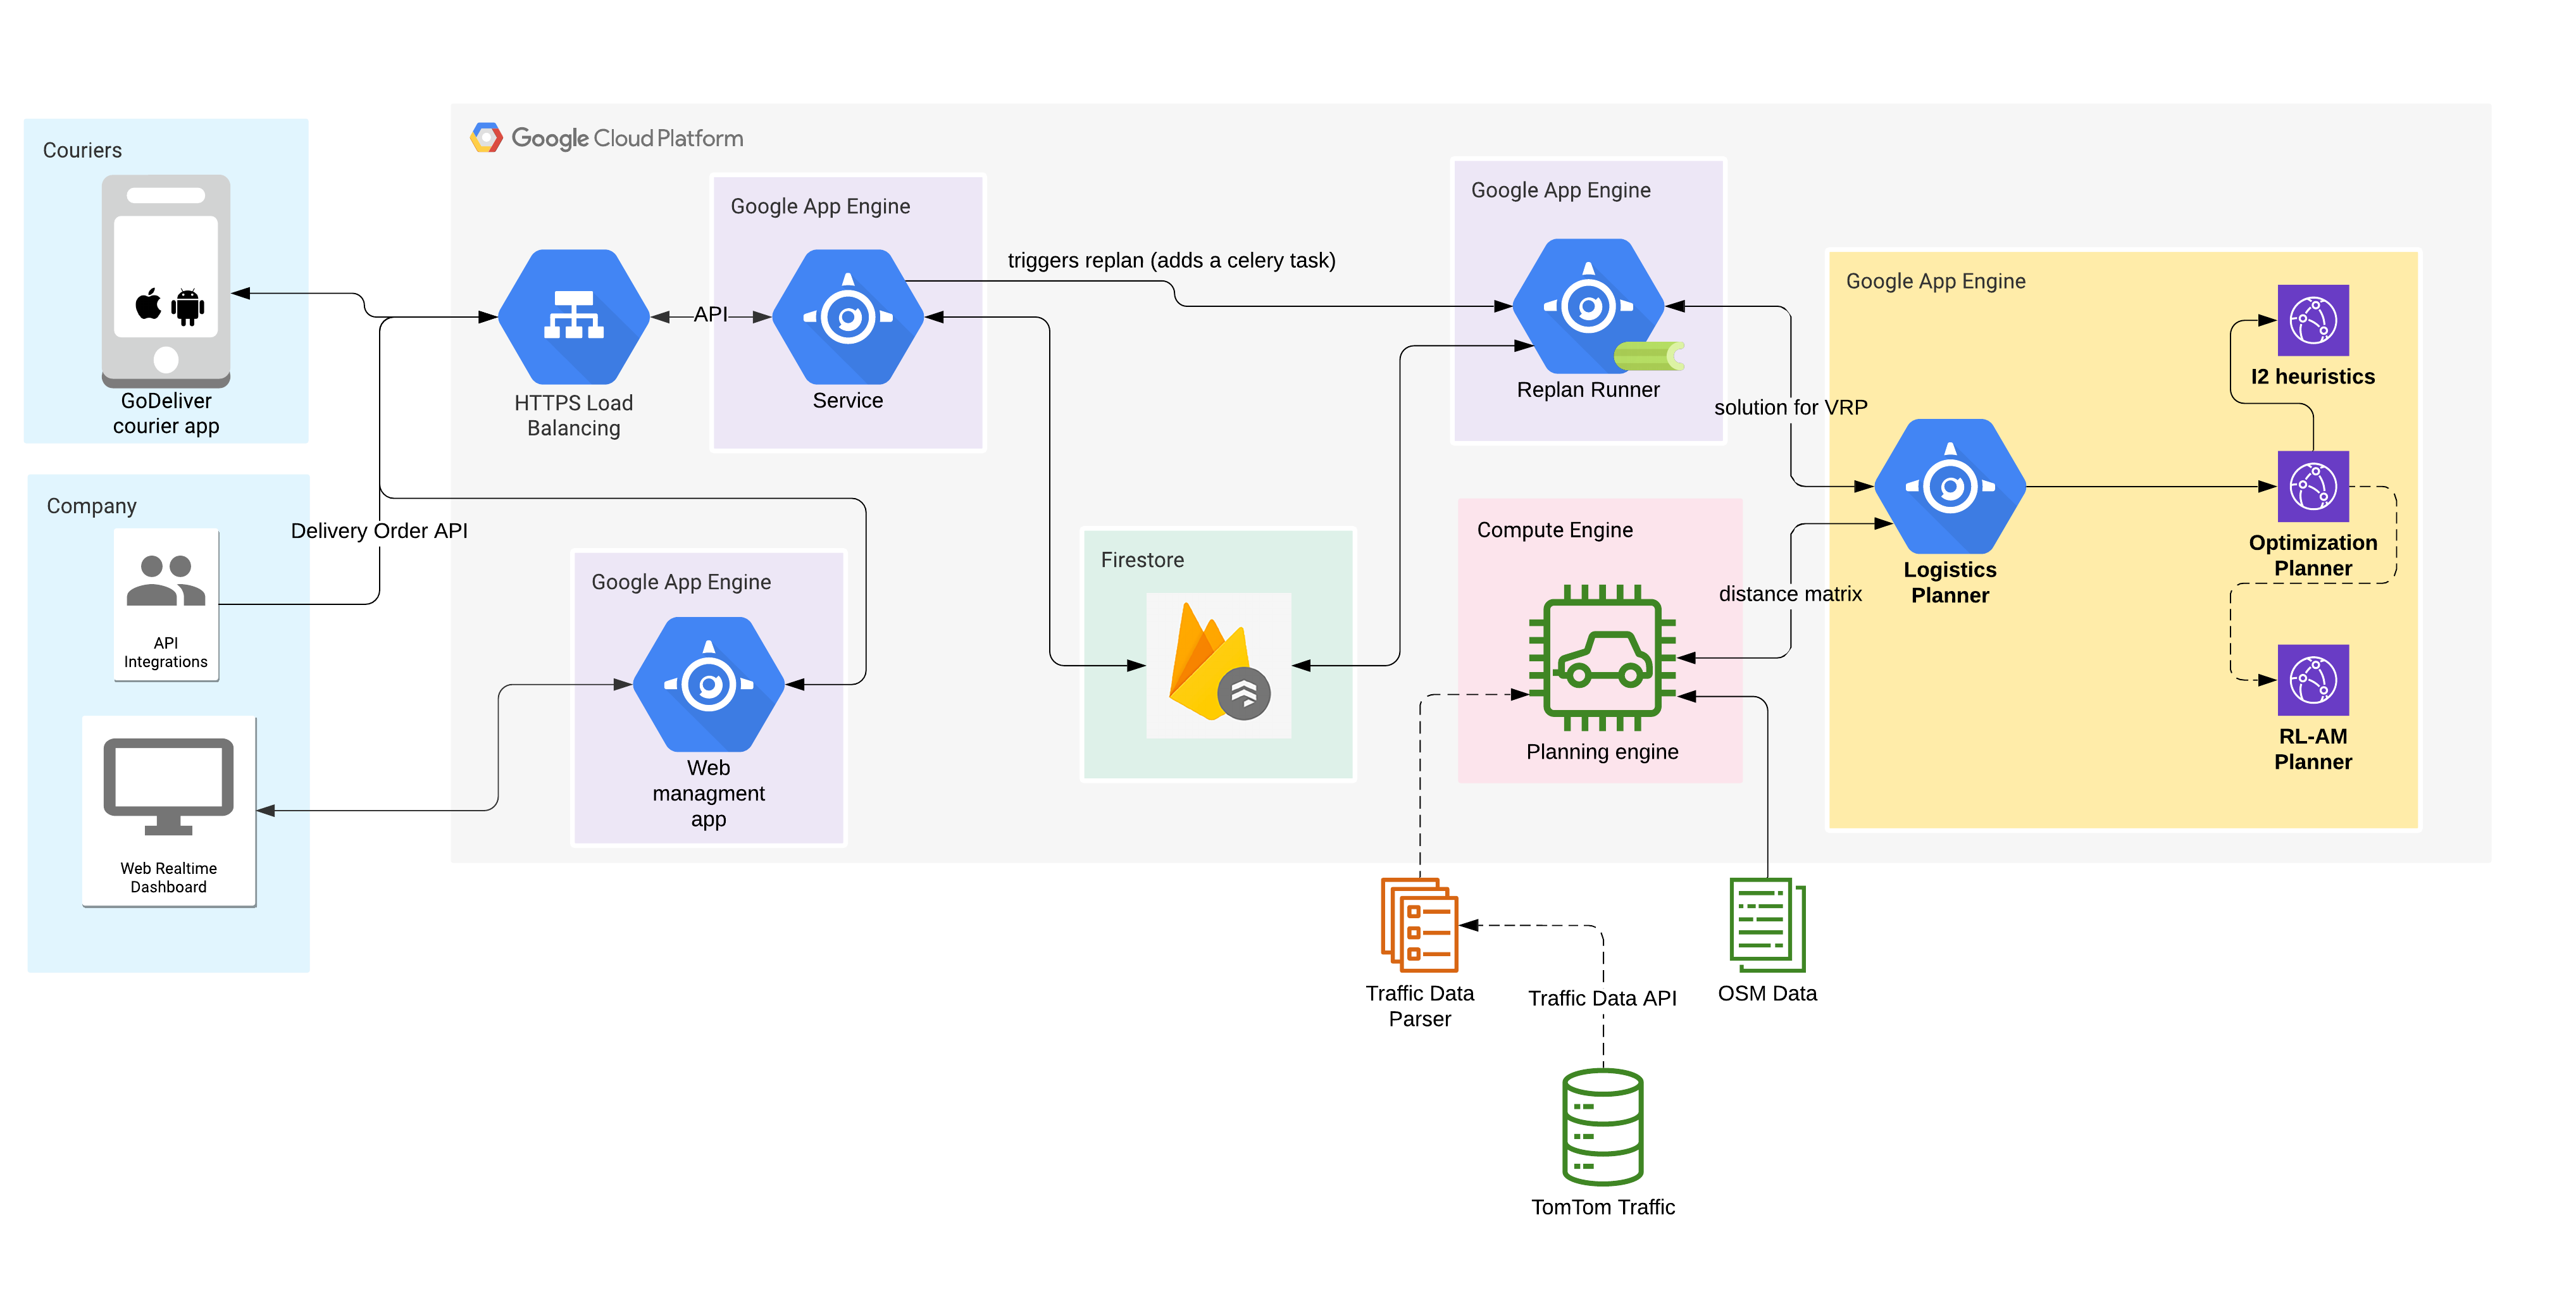
\includegraphics[width=1.0\textwidth]{resources/implementation/godeliver-system.png}
    \caption{GoDeliver System Architecture}
    \label{fig:godeliver-system}
\end{figure}

\subsection{Planning process}
The planning process is a complex operation which requires to work asynchronously because the planning of delivery orders is a time-consuming operation. The modern delivery planners have to support dynamic rescheduling and autonomously act upon the constantly changing environment.

The first part of the planning process is the creation of a delivery order, which is a request for delivery via API. The delivery order is saved in the database by GoDeliver Service with additional meta-data about the delivery state, etc. The database is monitored for a so-called \textit{trigger changes} which fires a replanning job via a distributed task queue Celery\footnote{\url{https://github.com/celery/celery}}. The \textit{trigger changes} are a list of actions such as creation of a new delivery order, changes in courier capacity, or a significant delay of delivery.

If such a replanning job is created, it is saved in Celery queue which is processed by GoDeliver Replanning Service \ref{fig:godeliver-system}. The replanning service loads a business configuration, delivery orders, and delivery plans from the database. It transforms the data into a generic structure which is accepted by our another service logistics planners that are solving the vehicle routing problem. The generic plan structure for the logistics planner freezes some delivery points which should not be considered by the planner since we do not want to change the current in-progress delivery points. This process is enabling us to perform the dynamic vehicle routing problem \ref{dynamic}.

Based on the business config, the desired vehicle routing solver is invoked via the logistics planner API. Usually, the planner takes the previous delivery plan and performs a heuristic algorithm like insertion heuristic which outputs an extended feasible plan. This plan is then improved by a local search algorithm to improve its cost function. Then the solution is processed by GoDeliver Replanning Service and saves the new delivery plans into the database.

\begin{figure}[ht]
    \centering
    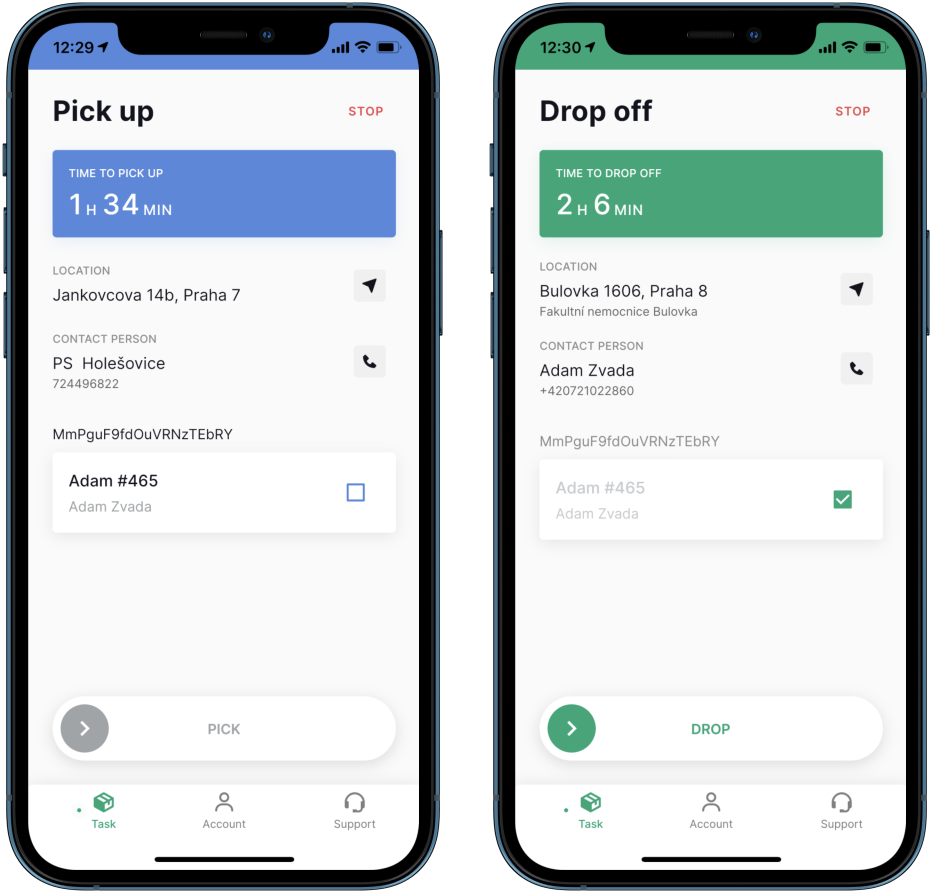
\includegraphics[width=0.75\textwidth]{resources/implementation/godeliver-app.png}
    \caption{GoDeliver Driver App}
    \label{fig:godeliver-app}
\end{figure}

In the future, the proposed \gls{vrptw} \gls{ai} planner will be used instead of insertion heuristics because we expect the \gls{ai} planner will outperform the insertion heuristics. The downside is that \gls{ai} planner is not able to leverage on the previous solution, which can lead to drastic changes in the solution structure of the delivery plan. However, this side effect is not a blocker since couriers only see one current delivery point from the delivery plan via GoDeliver mobile app \ref{fig:godeliver-app}.

\subsection{Planning Requirements}
The GoDeliver objective is to provide the most advanced and versatile urban logistics system. The logistics cases are always different for individual businesses and in order to cover them all we require a flexible but yet powerful planning system. For a new planner to be successfully used in the production environment, we have defined the planner requirements which have to be supported \ref{tab:vrptw-feature}. 

In the table \ref{tab:vrptw-feature}, we have summarized the supported features of our proposed \gls{vrptw} \gls{ai} It does not support features such as Pick and Deliver, predefined number of vehicles, and distance matrix. The Pick and Delivery is possible to support by extending the model to support a heterogeneous fleet based on this paper by J. Li et. al \cite{pick-deliver-ai} which extends the masking mechanism and \gls{rl} state and action to support the pick and deliver constraints. Distance matrix could be indirectly supported by applying multidimensional scaling \cite{multidimensional-scaling} to project the distance matrix into Euclidean space which is supported by the model. To define a fixed number of vehicles for a given \gls{vrptw} instance is surprisingly more complicated, but we propose that it can be achieved by implementing the support of multiagent reinforcement learning \cite{multiagent-rl} where each agent is one vehicle.

\begin{table}
     \centering
     \begin{tabular}{||c | c||} 
     \hline
     Feature & Is supported? \\ [0.5ex] 
     \hline\hline
     Time windows & \checkmark \\ 
     \hline
     Soft constraint & \checkmark \\
     \hline
     Distance matrix & indirectly\footnote{Multidimensional scaling \cite{multidimensional-scaling}} \\
     \hline
     Pick and Deliver & - \\
     \hline
     Demand Capacity & \checkmark \\ 
     \hline
     Balanced load across vehicles & \checkmark \\ 
     \hline
     Predefined number of vehicles & - \\ [1ex] 
    \hline
    \end{tabular}
    \caption{VRPTW AI support of planner requirements}
    \label{tab:vrptw-feature}
\end{table}

\section{Tech Stack - VRPTW via Optimization}

The planners based on optimization heuristics are implemented in programming languages Python\footnote{\url{https://python.org/}} and Go\footnote{\url{https://golang.org/}}.

\section{Tech Stack - VRPTW via AI}

The \gls{vrptw} planner via \gls{ai} is implemented in the programming language Python which is the most favorite programming language for any \gls{ai}-related project \cite{stack-overflow}. Besides it is easy language to get start with, it has many amazing \gls{ai} and data libraries such as Pandas, Numpy, Tensorflow or PyTorch.

Production implementation of neural network is developed with the use of deep learning frameworks. TensorFlow\footnote{\url{https://pytorch.org/}} and PyTorch\footnote{\url{https://pytorch.org/}} are the two most popular frameworks. It is an important decision which deep learning framework to choose if you plan to develop a production ready \gls{ml} pipeline.

\begin{figure}[ht]
    \centering
    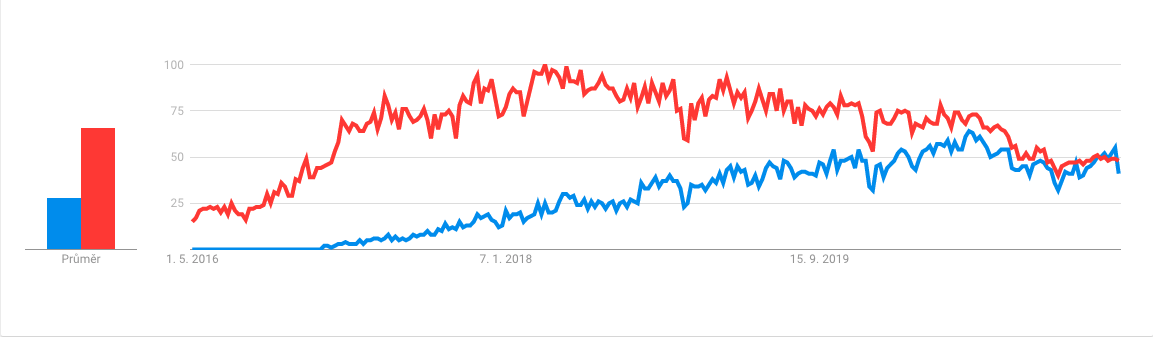
\includegraphics[width=1.0\textwidth]{resources/implementation/dp-framework-trend.png}
    \caption{Google Trend of PyTorch (blue) vs Tensorflow (red)}
    \label{fig:dp-framework-trend}
\end{figure}

The Google Trends graph \ref{fig:dp-framework-trend} shows how TensorFlow was more popular in the past, but lately they have similar amount of search results. However, the majority of the new research papers are implemented via PyTorch \cite{pytorch-data}. It is due to the fact that PyTorch has a great and intuitive API based on Numpy\footnote{\url{https://numpy.org/}} operations and it is even slightly faster than TensorFlow.

In this thesis, we have decided to use PyTorch as our main deep learning framework.



    \chapter{Evaluation}

In this chapter, we will evaluate our proposed planning model based on deep reinforcement learning built upon Transformer \ref{transformer} architecture utilizing Graph Attention Network \ref{graph-attention-network} and benchmark the performance against constructive heuristics and metaheuristics.

\section{Dataset}
The dataset used for training and evaluation was generated on the fly via a uniform probability distribution within a given range. The reason we decided to generate the data is that learning reinforcement policy requires a large amount of training data. Since it learns by interacting with the environment, we do not need labeled datasets and generating them seems as the best approach. Nevertheless, in further work, the model will require other kinds of distribution to simulate a real-world demand.

In real-world routing applications, the geographic coordinate system is typically used for specifying locations. However, our proposed model requires locations between $[0, 1]$ to achieve model convergence. The locations of depots and delivery nodes were generated via uniform distribution within a range of $[0, 1] \times [0, 1]$.

The data for the demand capacity of a delivery node is a discrete number $\{1, \cdots, 9\}$ chosen uniformly at random with assumption that the depot has a demand capacity of zero. 

Lastly, each location has assigned time windows that work as a soft constraint at which time a vehicle is supposed to visit the node. We generate different lengths of time windows based on the problem size (20, 50, 100). For the problem size of 20 nodes, the time window value occurs in a range of $\{0, \cdots, 10\}$ with the condition that the length of the time window is less than four. The problem size of 50 nodes has the upper bound set to 20 with a maximal length of 6 and the case of 100 nodes, the upper bound is 40 and the maximal window length is 9. Similarly, the start and end of a time window are generated with uniform distribution.

\section{Sample Solutions}
To better imagine the complexity and variability of solving \gls{vrptw}, in Figure \ref{fig:sample-20} and \ref{fig:sample-50} we illustrate a random solution predicted by our proposed deep learning model. On the left, we visualize the customer's time windows using Gantt diagram and on the right are shown the routes for each vehicle. Each color represents a vehicle which servers the customers represented by a node with a generated time window.

\begin{figure}[ht]
    \centering
    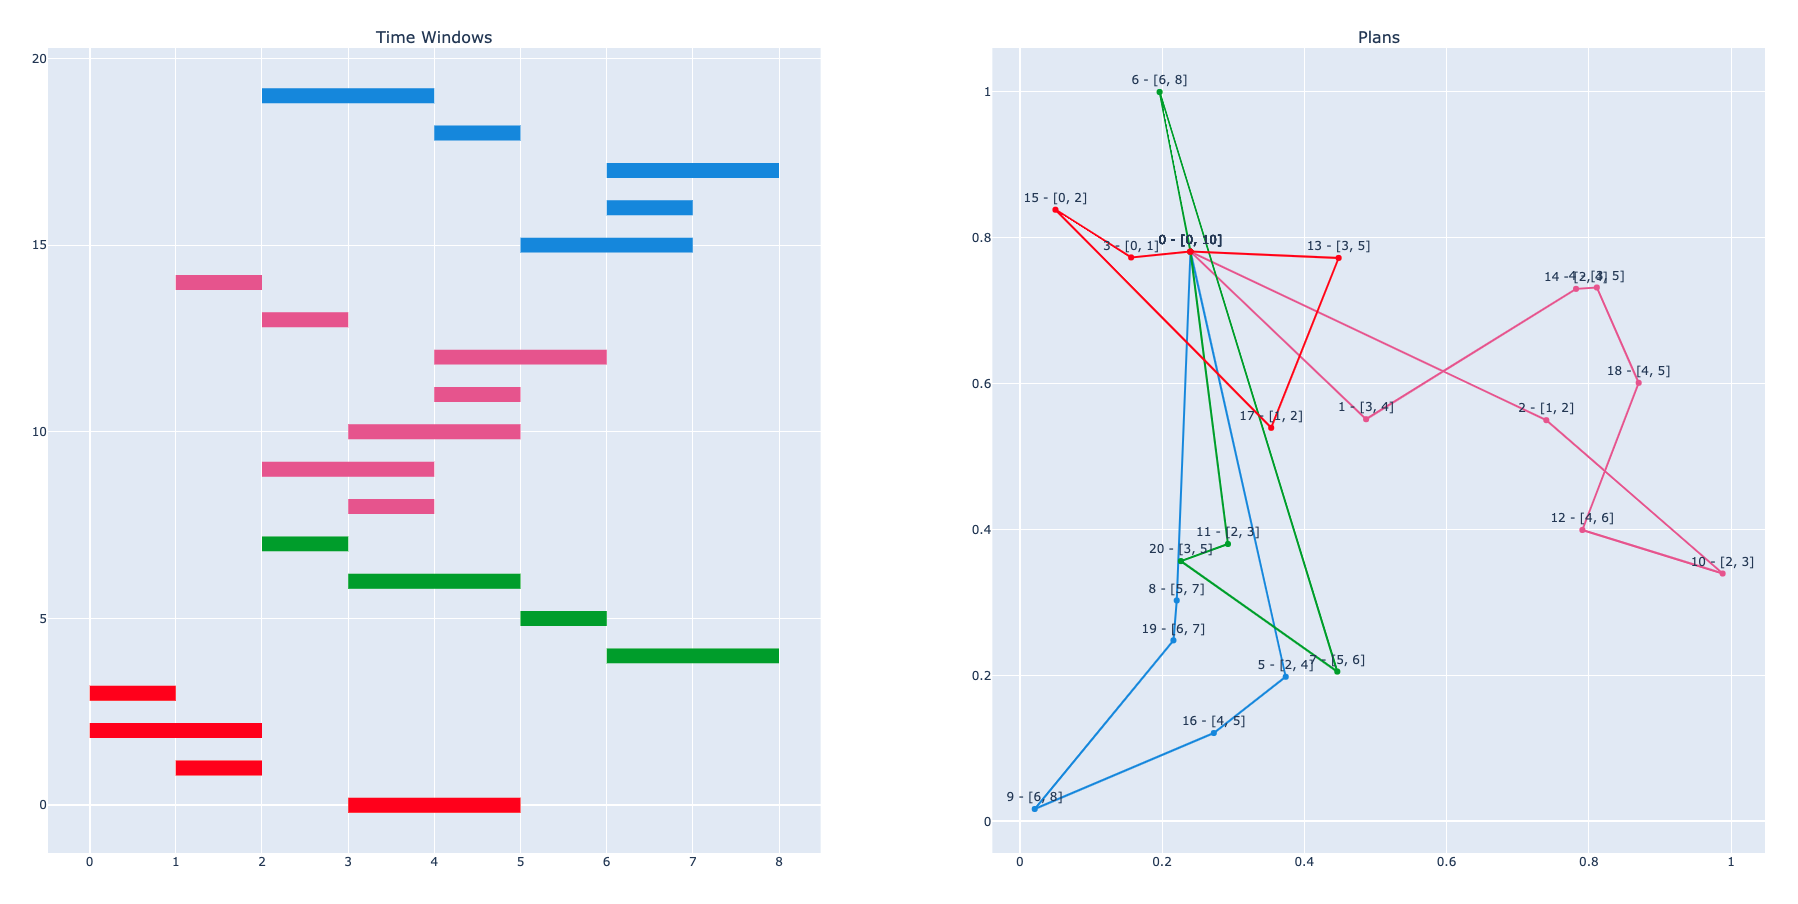
\includegraphics[width=1.0\textwidth]{resources/evaluation/sample-20.png}
    \caption{Sample solution of random \gls{vrptw} instance for problem size 20.}
    \label{fig:sample-20}
\end{figure}

The \gls{ai} model has to optimize the route path with focus to minimize the travelled distance, but simultaneously early and late arrivals should be avoided. Our model is able to solve \gls{vrptw} instance considers both distance and time window constrains. The windows are soft constrained, which results in a much larger combinatorial space of possible solutions than considering just hard constrained time windows. As illustrated on Figure \ref{fig:sample-50} the model sometimes sacrifices the time of a served customer in order to optimize the route distance and vice versa.

\begin{figure}[ht]
    \centering
    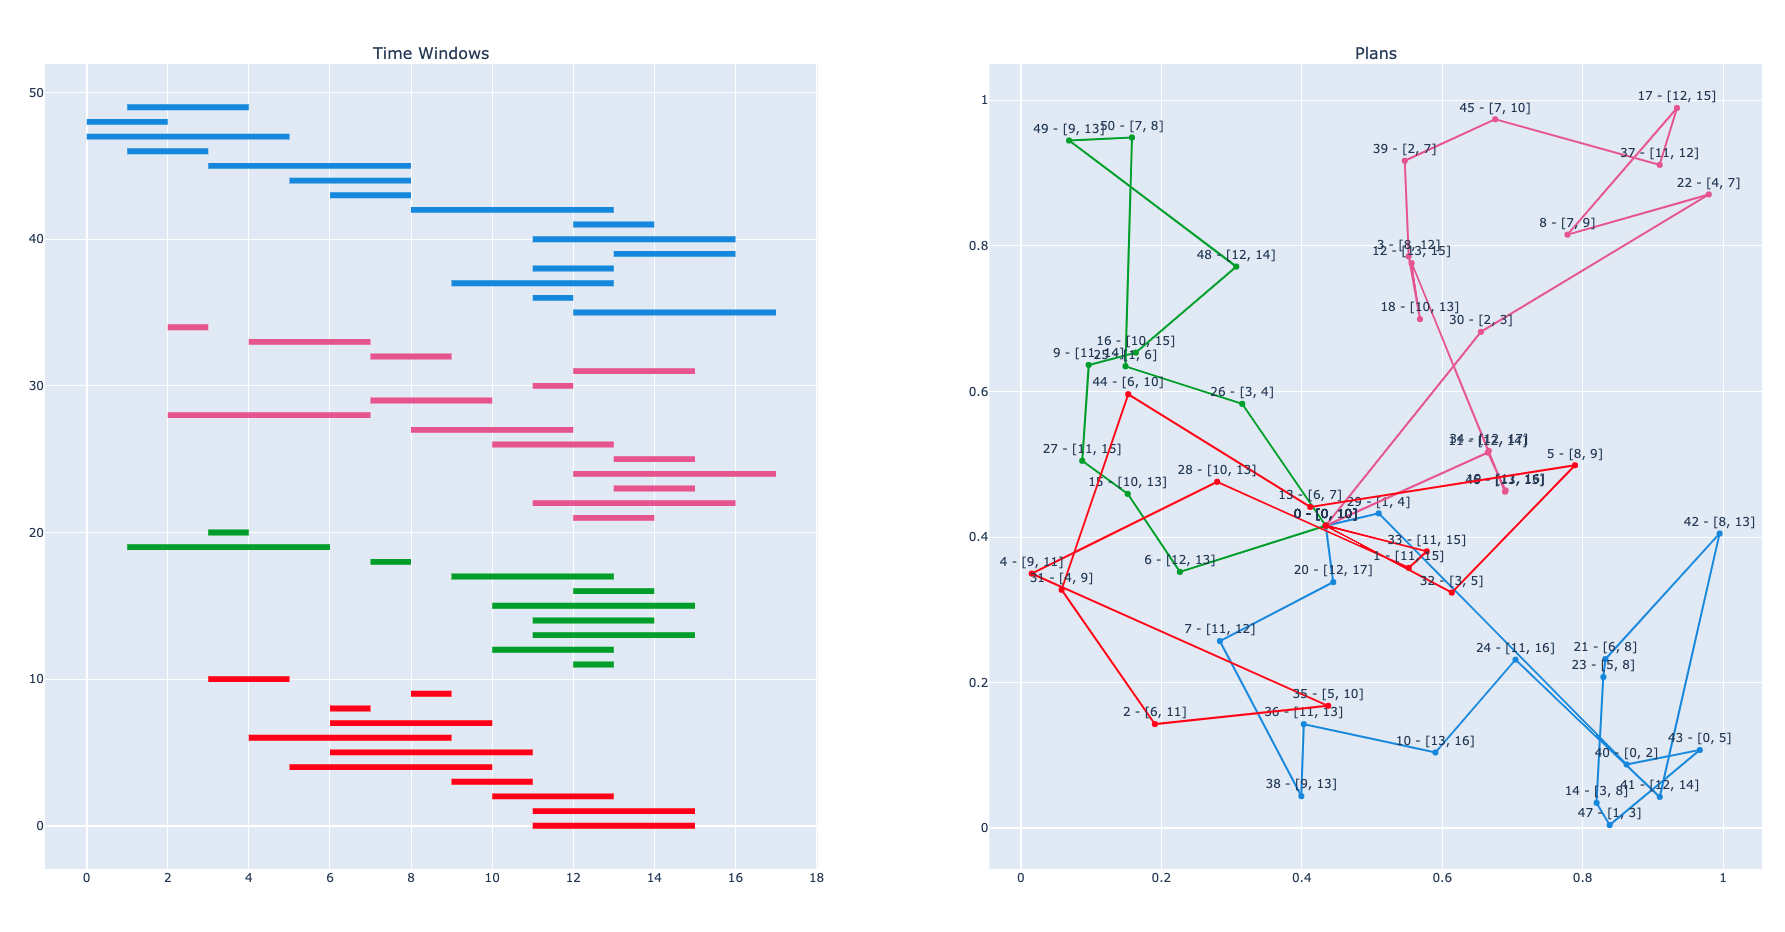
\includegraphics[width=1.0\textwidth]{resources/evaluation/sample-50.png}
    \caption{Sample solution of random \gls{vrptw} instance for problem size 50.}
    \label{fig:sample-50}
\end{figure}

The model has successfully learned the policy how to pick the next node to visit, the time windows are almost cascadingly sorted, and the routes are suboptimally optimized based on distance. However, it is clearly not an optimal solution, but it proves that the problem of vehicle routing with soft constrained time windows is possible to be solved with \gls{ml} and the research is on the right path to outperform regular metaheuristics. In the section \ref{benchmarking} we compare the model with our implemented constructive heuristics and metaheuristics

\section{Experiments}
\subsection{Time Windows}
The main goal of this thesis was to integrate the soft constraint of time windows to \gls{vrp} model introduced by Kool et al.\cite{attention-route}. The model is extended by our proposed cost function \ref{vrptw-cost} that penalizes early and late arrivals. The early arrival is not as crucial as delayed visit, so we have decided that the penalty for early arrival is always less than late visit $p_e < p_l$.

\begin{figure}[ht]
    \centering
    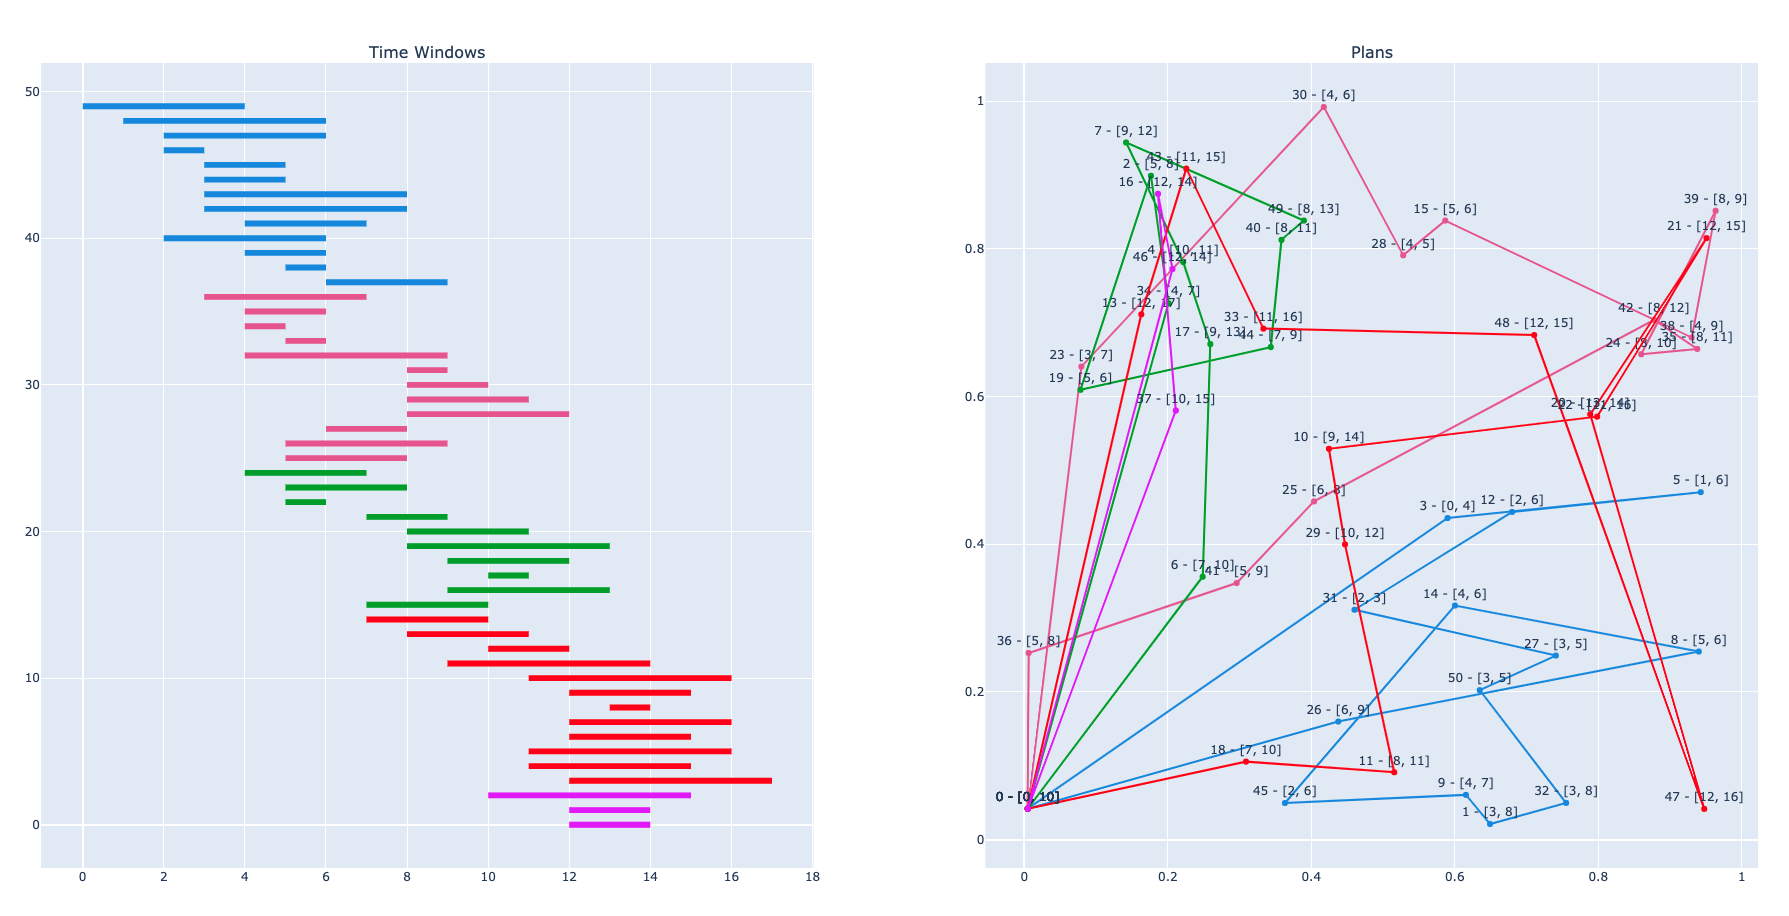
\includegraphics[width=1.0\textwidth]{resources/evaluation/tw-problem.png}
    \caption{Low penalty for early visit of node results in poor performance.}
    \label{fig:tw-problem}
\end{figure}

Finding a proper penalty values $p_e$ and $p_l$ for time windows is one of the most important steps because an incorrect penalty highly influences the model in choosing the next node to visit.

The Figure \ref{fig:tw-problem} illustrates how the performance is degraded by choosing an incorrect penalty value for early arrival $p_e$. If the early penalty is too low, the model will strictly focus on minimizing the late arrival and Gantt diagram of time windows looks like a plan for just a single vehicle.

We have empirically tested various kinds of penalties and updated them based on our observations. After the experiments, we have chosen $p_e = 0,25$ and $p_l  = 0,5$ which resulted in predicting a feasible plans with properly distributed time windows across the vehicles as shown in Figure \ref{fig:nice-tw}.

\begin{figure}[ht]
    \centering
    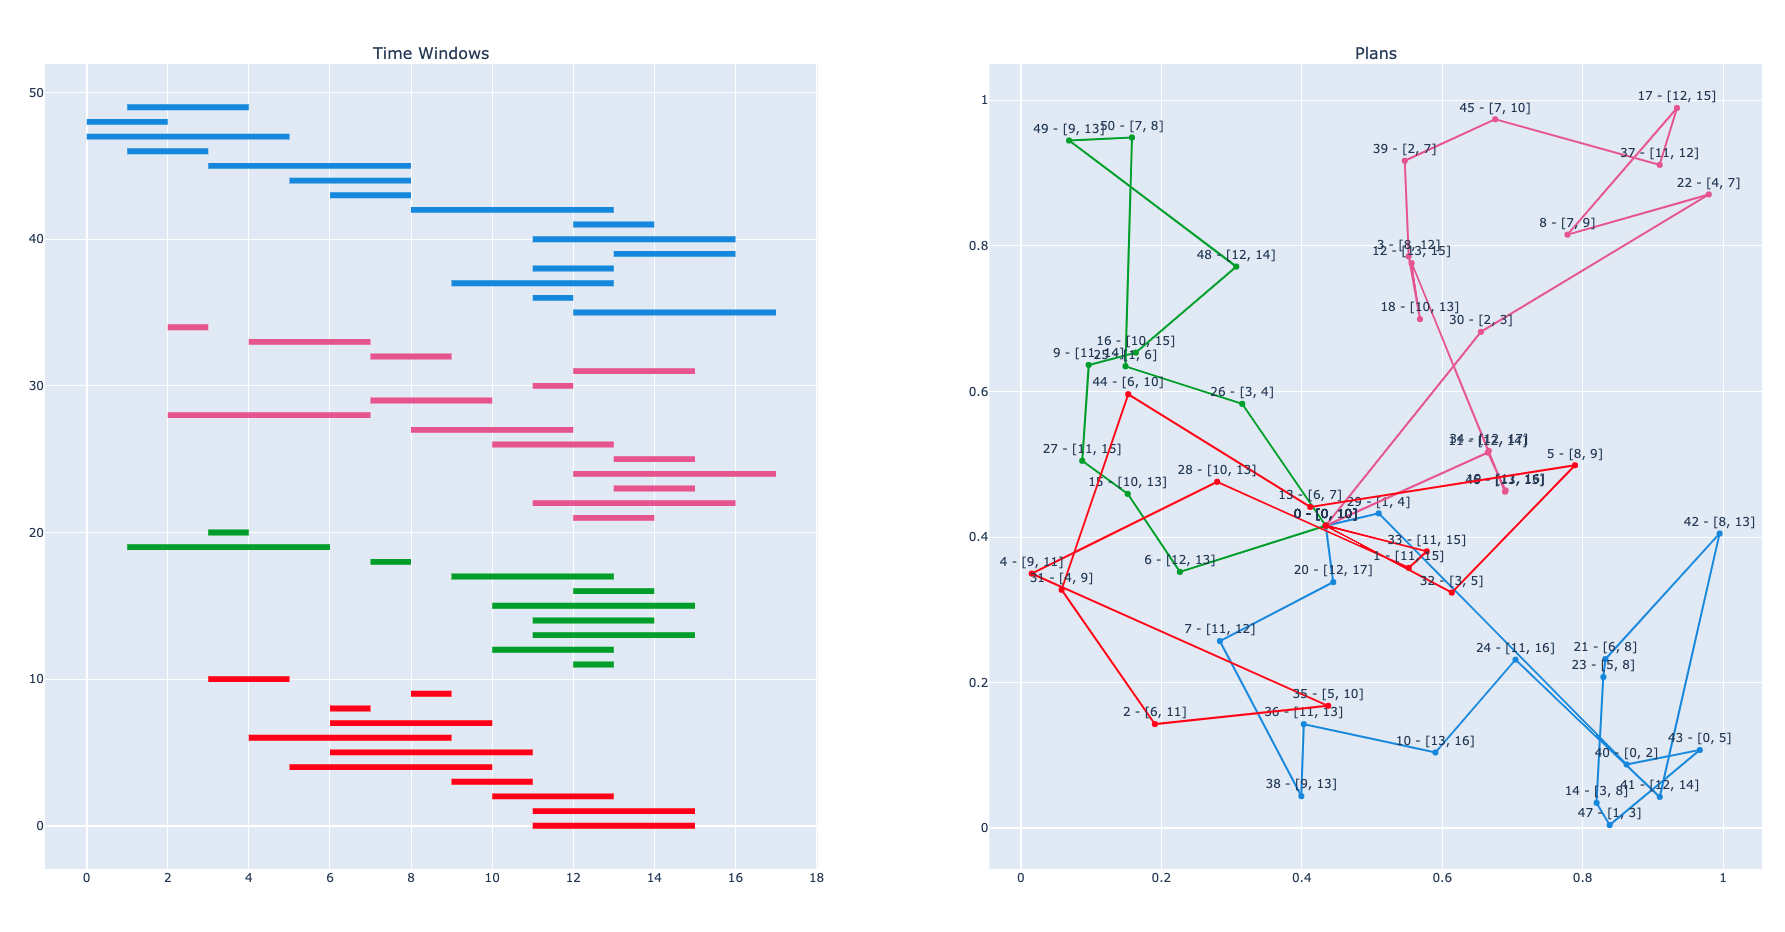
\includegraphics[width=1.0\textwidth]{resources/evaluation/sample-50.png}
    \caption{Properly distributed time windows across the vehicles.}
    \label{fig:nice-tw}
\end{figure}

\subsection{Balancing Plans}
In real-world solution of \gls{vrp}, we aim to balance the number of served customers across vehicles. It means the number of nodes in a given route is supposed to be uniformly distributed across all routes. However, we have noticed that the model was constantly adding additional routes of size one as illustrated on Figure \ref{fig:unbalanced}.

\begin{figure}[ht]
    \centering
    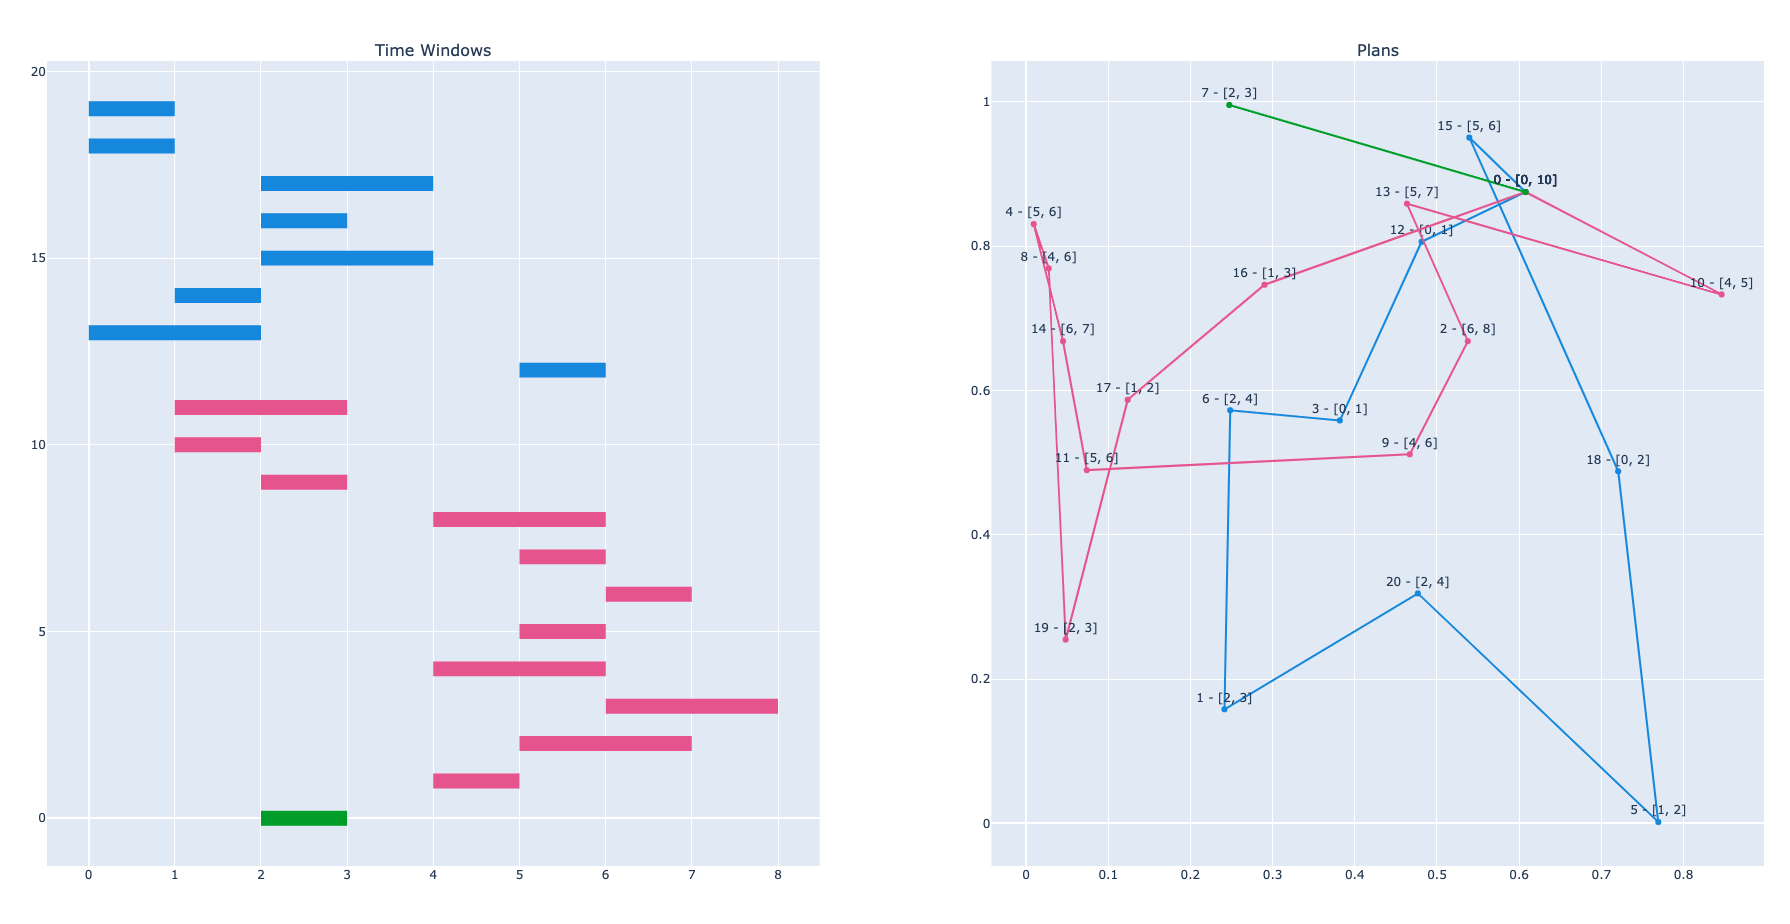
\includegraphics[width=1.0\textwidth]{resources/evaluation/unbalanced-plan.png}
    \caption{Unbalanced delivery plans.}
    \label{fig:unbalanced}
\end{figure}

Therefore, we have decided to penalize the delivery plans that are not balanced by including an unbalance penalty. We calculate the standard deviation of plans with the objective to be minimized using our cost function. This approach helped in creating balanced delivery plans.

\subsection{Generalization}
A great downside of this proposed model is its sensitivity to data input, which results in poor model generalization. If we introduce to a model a distribution of data which has not been seen before, it is not possible to predict sensible delivery plans and the model just serves each of the nodes by a single vehicle. This behavior is shown in Figure \ref{fig:model-breaks}. The model has even problems with generalization to different input data distributions in a single dataset.

\begin{figure}[ht]
    \centering
    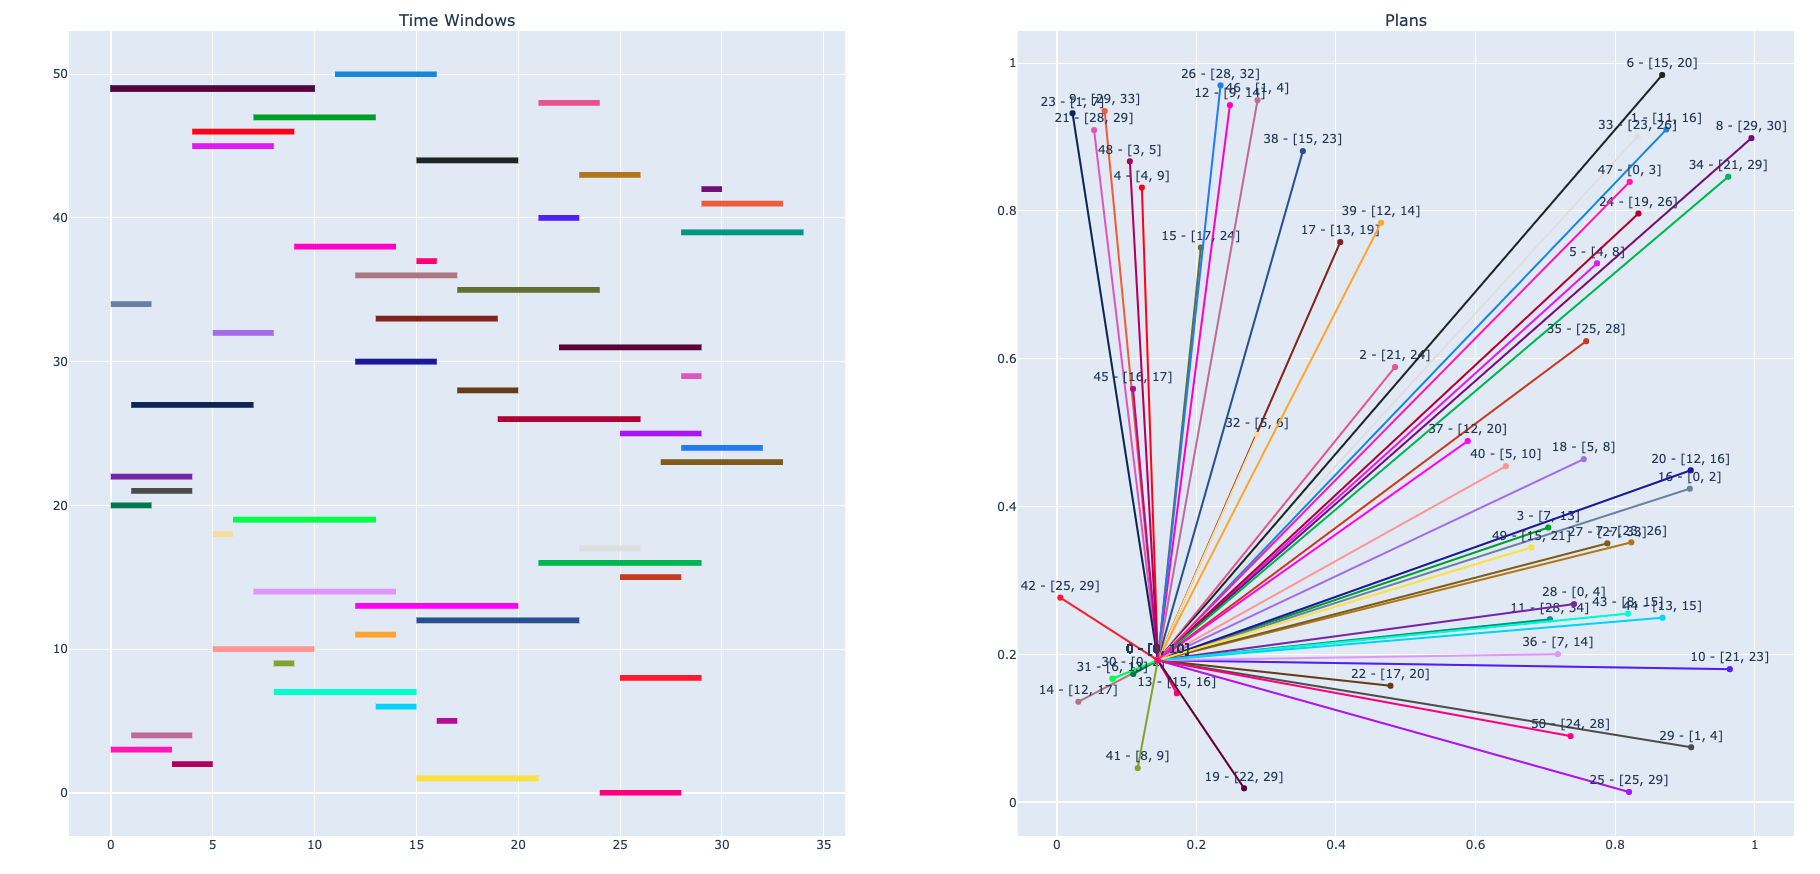
\includegraphics[width=1.0\textwidth]{resources/evaluation/data-sensitivity.png}
    \caption{If the model does not know how to solve the instance, it just sends each vehicle to serve one node.}
    \label{fig:model-breaks}
\end{figure}

Another model sensitivity is to the instance problem size. If the model is trained on the problem size of 20 nodes, the model performance is continuously degraded by a larger difference of the problem size on which it was trained on. We tried training the model on a dataset of different problem sizes, but the network was not effectively learning. The model has to be trained on a problem size with a minimal difference.

The solution is to train multiple models for each of the problem sizes and data distribution. However, this seems as a great obstacle in using this model in real-world environment and thus a new model with improved model generalization needs to be proposed by researches.

\subsection{Training Process}

The training process of such a network is very time consuming and with our limited available hardware, the \gls{vrptw} model for solving 50 nodes requires at least 5 days to be fully trained. Therefore, experimenting with a different values of network hyperparameters is not part of this thesis. We only focused on proving if even such a problem like \gls{vrptw} can be sub-optimally solved via \gls{ml}. We have used the same hyperparameters as Kool et al. \cite{attention-route} in their research.

During the training process, we have observed multiple values of the cost function \ref{vrptw-cost} to understand if the network was successfully learning to solve the problem.

\begin{figure}[ht]
    \centering
    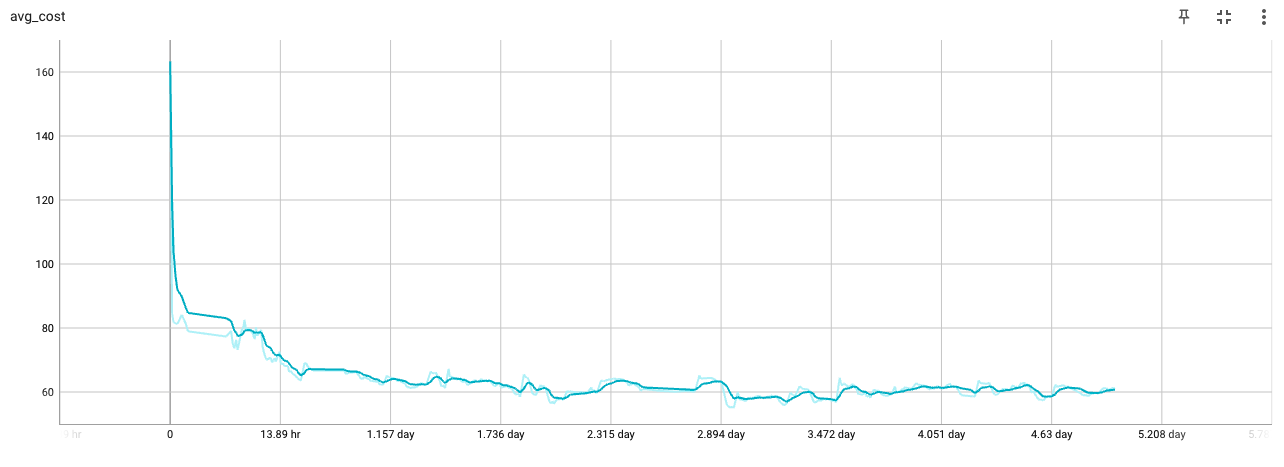
\includegraphics[width=0.75\textwidth]{resources/evaluation/avg-cost.png}
    \caption{Average cost (reward) per epoch on training data.}
    \label{fig:avg-cost}
\end{figure}

In Figure \ref{fig:avg-cost} we observe the average cost of the predicted solutions per epoch. It fairly quickly plateaued, but if we look at the average cost on the validation dataset \ref{fig:avg-cost-val}, the value was still decreasing. The model was still improving just on different parts of the cost function. 

\begin{figure}[ht]
    \centering
    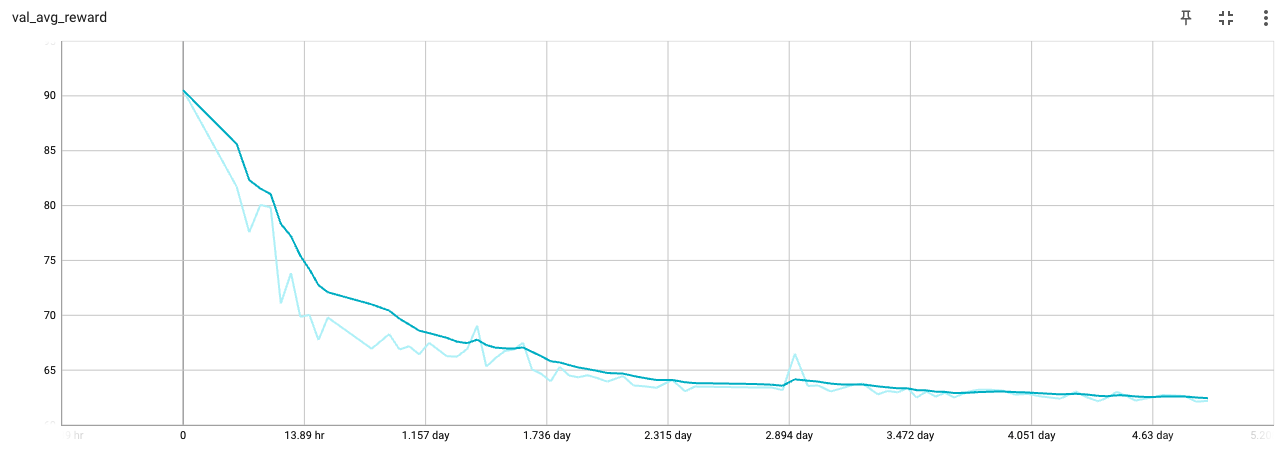
\includegraphics[width=0.75\textwidth]{resources/evaluation/val-avg-cost.png}
    \caption{Average cost (reward) per epoch on validation data.}
    \label{fig:avg-cost-val}
\end{figure}

If we would experiment with hyperparameter tuning, in this case, we could try to use the decaying learning rate which we assume would further more decreased the cost function.

\begin{figure}[ht]
    \centering
    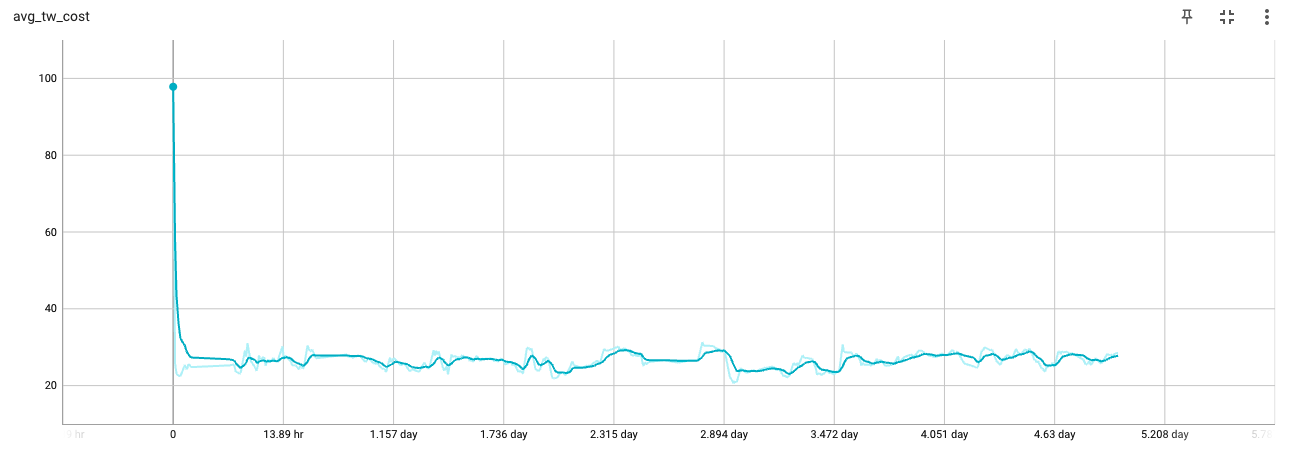
\includegraphics[width=0.75\textwidth]{resources/evaluation/avg-tw-cost.png}
    \caption{The average cost for time windows per epoch.}
    \label{fig:avg-cost-tw}
\end{figure}

In Figure \ref{fig:avg-cost-tw} we observe the average penalty for early and late arrivals of the predicted routes per epoch. The model quickly learns the policy strategy how to predict the next node to visit based on the time constraint. We assume that the model first learns the strategy for minimizing the time window based on the drastic drop of the time window cost function and then it learns to optimize the distance of routes. In Figure \ref{fig:avg-cost-distance} we observe the average total distance of predicted routes per epoch and the cost is constantly decreasing while the model learns to optimize the distance.

\begin{figure}[ht]
    \centering
    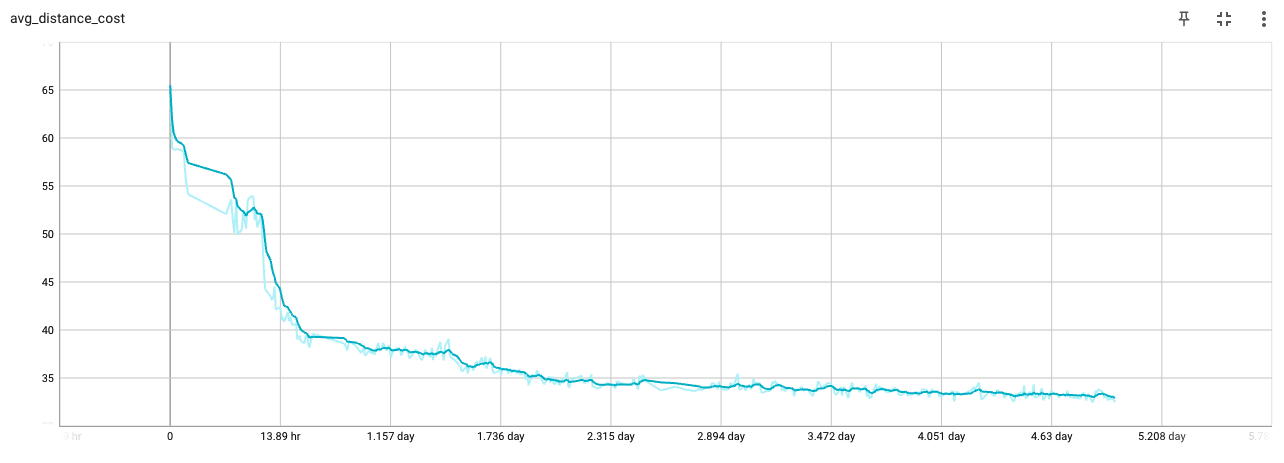
\includegraphics[width=0.75\textwidth]{resources/evaluation/avg-distance-cost.png}
    \caption{The average distance cost per epoch.}
    \label{fig:avg-cost-distance}
\end{figure}

In Figure \ref{fig:avg-cost-balance} is the last observed part of the cost function, the unbalance penalty, which is slowly decreasing while the model learns to distribute the nodes uniformly across the vehicles.

\begin{figure}[ht]
    \centering
    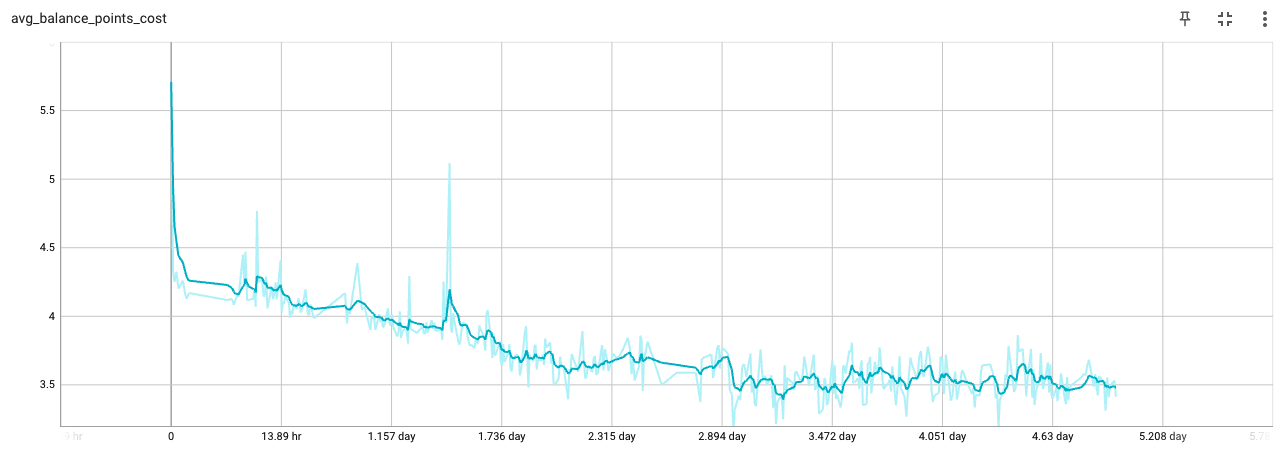
\includegraphics[width=0.75\textwidth]{resources/evaluation/avg-balance-cost.png}
    \caption{The average cost of balanced plans.}
    \label{fig:avg-cost-balance}
\end{figure}

The cost function is used as a reward function for \gls{rl}. It is important to note that the model can never achieve a value of the cost function which would converge to zero.
\newline

\section{Benchmarking}\label{benchmarking}
We know that our deep reinforcement learning model for sub-optimally solving \gls{vrptw} can predict a solution for \gls{vrptw} instances \ref{fig:sample-50}. However, to evaluate the model performance, we need to compare it with other reliable methods like constructive heuristics and metaheuristics.

The first benchmark is insertion heuristics \ref{insertion-heuristics} which produces a feasible solution in a matter of seconds. It is frequently used to generate an initial solution which is then optimized by a local search algorithm or population-based method. The second typical benchmark used in research papers is OR-Tools framework \ref{or-tools} and its is widely used for many optimization tasks. Lastly, the third benchmark combines insertion heuristics as an initial solution and OR-Tools planner as a metaheuristics.

\begin{table}[ht]
\centering
\resizebox{\textwidth}{!}{

\begin{tabular}{lrrrrr}
\toprule
{\textbf{Model}} & DistanceCost & DelayCost & EarlinessCost & ComputationTime & \textbf{AggCost} \\
{} &          Km &       min. &           min. &             sec &       \\
\midrule
\textbf{INSERTION\_HEURISTIC}    &           981 &          0 &            847 &                1 &    \textbf{1,193} \\
\textbf{RL\_AM\_PLANNER}          &           610 &         38 &            871 &                0.5 &      \textbf{847} \\
\textbf{OR\_TOOLS}               &           482 &          4 &            814 &              120 &      \textbf{687} \\
\textbf{OR\_TOOLS\_INSERTION}     &           488 &          1 &            798 &              121 &      \textbf{688} \\
\textbf{RL\_AM\_OR\_TOOLS\_PLANNER} &           482 &          4 &            814 &              120 &      \textbf{688} \\
\bottomrule
\end{tabular}

}
\caption{Benchmarking of VRPTW solvers for problem size of 20 nodes.}
\label{tab:result-20}
\end{table} 

In table \ref{tab:result-20} we may see the average cost of our implemented planners on 64 different \gls{vrptw} instances. 
The \textit{AggCost} is the same as being used in our model architecture \ref{vrptw-cost}.


\begin{table}[ht]
\centering
\resizebox{\textwidth}{!}{

\begin{tabular}{lrrrrr}
\toprule
{\textbf{Model}} & DistanceCost & DelayCost & EarlinessCost & ComputationTime & \textbf{AggCost} \\
{} &          Km &       min. &           min. &             sec &       \\

\midrule
\textbf{INSERTION\_HEURISTIC}    &         2,306 &          0 &          4,355 &               39 &    \textbf{3,395} \\
\textbf{RL\_AM\_PLANNER}          &         1,297 &        100 &          3,634 &                2 &    \textbf{2,255} \\
\textbf{OR\_TOOLS}               &           757 &        539 &          6,180 &              154 &    \textbf{2,571} \\
\textbf{OR\_TOOLS\_INSERTION}     &         2,007 &          3 &          3,967 &              192 &    \textbf{3,000} \\
\textbf{RL\_AM\_OR\_TOOLS\_PLANNER} &           759 &        537 &          6,161 &              156 &    \textbf{2,568} \\
\bottomrule
\end{tabular}


}
\caption{Benchmarking of VRPTW solvers for problem size of 50 nodes.}
\end{table} 


\begin{table}[ht]
\centering
\resizebox{\textwidth}{!}{

\begin{tabular}{lrrrrr}
\toprule
{\textbf{Model}} & DistanceCost & DelayCost & EarlinessCost & ComputationTime & \textbf{AggCost} \\
{} &          Km &       min. &           min. &             sec &       \\
\midrule
\textbf{INSERTION\_HEURISTIC}    &         4,654 &          0 &         17,548 &              750 &    \textbf{9,041} \\
\textbf{RL\_AM\_PLANNER}          &         5,852 &          1 &         15,805 &               16 &    \textbf{9,804} \\
\textbf{OR\_TOOLS}               &         1,034 &      2,885 &         23,719 &              199 &    \textbf{8,406} \\
\textbf{OR\_TOOLS\_INSERTION}     &         4,478 &          0 &         17,109 &              807 &    \textbf{8,755} \\
\textbf{RL\_AM\_OR\_TOOLS\_PLANNER} &         1,034 &      2,885 &         23,719 &              219 &    \textbf{8,406} \\
\bottomrule
\end{tabular}
}
\caption{Benchmarking of VRPTW solvers for problem size of 100 nodes.}
\end{table} 



    \begin{conclusion}
    The thesis objective was to explore if vehicle routing problem (\gls{VRP}) with time windows can be solved via machine learning.
\end{conclusion}

    
    % bibliography
    \bibliographystyle{prefs/iso690}
    \bibliography{ref}
    
    \appendix
    
    % acronyms
    \printglossaries
    
    % media contents
    \chapter{Media contents}\label{app:CDcontent}
    \begin{figure}
    	\dirtree{%
    		.1 readme.txt\DTcomment{the file with CD contents description}.
    		.1 data\DTcomment{the data files directory}.
    		.2 example\textunderscore sequence\DTcomment{the directory with example sequence from dataset}.
    		.3 *.jpg\DTcomment{the example images}.
    		.2 example\textunderscore sequence\textunderscore graphs\DTcomment{the directory of graphs of experiments}.
    		.3 *.png\DTcomment{the motion output graphs}.
    		.2 tracking\textunderscore example.mp4\DTcomment{the example video file}.
    		.1 src\DTcomment{the directory of source codes}.
    		.2 models\DTcomment{the directory of deep learning modules}.
    		.2 utils\DTcomment{the directory of helper modules}.
    		.2 *.py\DTcomment{the Python source files}.
    		.1 text\DTcomment{the thesis text directory}.
    		.2 thesis\DTcomment{the directory of \LaTeX{} source codes of the thesis}.
    		.2 thesis.pdf\DTcomment{the Diploma thesis in PDF format}.
    	}
    \end{figure}
    

\end{document}
